\documentclass[11pt]{article}
\usepackage[margin=1in]{geometry}
\usepackage{amsmath,amssymb,amsthm}
\usepackage{boldtensors}
% boldtensors declares the symbol font `cmbboard' from the bbold family, which
% is not present in every TeX installation (it aborts at the start of math
% mode). Redirect it to the always-available AMS `msb' family; the `"'-syntax
% that would actually render a cmbboard glyph is unused here, so this only
% removes the missing-font dependency.
\DeclareSymbolFont{cmbboard}{U}{msb}{m}{n}
\usepackage{hyperref}
\usepackage{booktabs}
\usepackage{enumitem}
\usepackage{graphicx}

\newcommand{\dd}{\mathrm{d}}
\newcommand{\norm}[1]{\lVert #1 \rVert}
\newcommand{\code}[1]{\texttt{#1}}
\newcommand{\jump}[1]{[\![#1]\!]}
\emergencystretch=3em

\title{Schwarz Coupling for Solid Dynamics in Norma.jl:\\
Transmission Conditions, Interface Energy,\\
and Energy-Consistent Design}
\author{Alejandro Mota}
\date{July 2026}

\begin{document}
\maketitle

\begin{abstract}
This note is the consolidated reference for the Schwarz coupling conditions
implemented in Norma.jl and for the study of their energy behavior in
dynamic solid mechanics. On a shared (nonoverlap) interface, the Robin
condition is fully reflecting and the impedance condition is absorbing, with
the impedance fixed by material data. On an overlap boundary, the impedance
condition is consistent with the monodomain solution only when it carries
the partner traction; with the consistent nodal traction the coupling is
exact on conforming meshes (energy error $59\% \to 0.08\%$ over $1$\,ms,
with no adjustable parameters). On nonconforming meshes the overlap coupling
cannot be assigned a reliable energy budget: because the two sides transfer
partner data through independent, non-adjoint operators, the interface work
is sign-indefinite --- measured drifts swing from $-53\%$ to $+174\%$ to
$-66\%$ across adjacent mesh ratios --- and at a ten-millisecond horizon
$74$ of $108$ configurations fail by element inversion after exponential
energy growth. Every remedy attempted at the interface --- variational
transfer, exact traction transfer, filtered dissipation --- fails for a
structural reason: the persistent interface jump is a disagreement between
the two grids' discrete dispersion relations, not a transfer defect. Energy
consistency requires a single-valued interface traction acting through
$L^2$-adjoint transfer operators, which makes the interface power telescope
to a sign-definite dissipation on the interface jump; this construction is
available only on the nonoverlap variant, whose two sides share one
interface. The resulting adjoint-paired nonoverlap coupling --- one shared
cross-mass matrix, force transfers adjoint to the partner's kinematic
transfers, a harmonic-mean pair impedance, the dynamically consistent
d'Alembert interface reaction, and an implicit--explicit treatment of the
interface rows for explicit subdomains --- never injects energy at any mesh
ratio, conserves energy to $0.3\%$ over $1$\,ms in all four integrator
combinations on conforming and mildly nonconforming meshes, and holds the
monodomain trajectory over ten thousand steps. The note also records the
subcycled (multi-time-step) exchange, the measured incompatibility of exact
interface-work telescoping with a partitioned iteration, and the slot-keyed
relaxation state required when controller stops exceed a subdomain time
step. Practical recommendations and open questions close the note.
\end{abstract}

\medskip
\noindent\emph{This document consolidates and supersedes three earlier notes:
``Impedance-Matching vs.\ Robin--Robin Coupling Conditions in Schwarz
Methods,'' ``Variational Transfer for Impedance-Overlap Schwarz on
Non-Conforming Meshes,'' and ``Interface Energy Loss of the Impedance-Overlap
Schwarz Coupling on Nonconforming Meshes, and an Energy-Consistent
Redesign'' (June--July 2026).}

\tableofcontents

\section{Setting}
\label{sec:setting}

\subsection{Decompositions and notation}

Consider a solid body $\Omega \subset \mathbb{R}^3$ decomposed into two
subdomains $\Omega_1$ and $\Omega_2$ that are integrated independently and
coupled by a Schwarz iteration. Norma.jl supports two geometric
configurations.

\paragraph{Nonoverlap.} The subdomains partition $\Omega$ and share an
interface $\Gamma = \partial\Omega_1 \cap \partial\Omega_2$ on which coupling
is imposed. Let $~n_k$ be the outward unit normal to $\Omega_k$ on $\Gamma$
(so $~n_1 = -~n_2$) and let $~t_k = ~\sigma_k\,~n_k$ denote the traction on
$\Omega_k$'s side. Continuity of the coupled solution requires
\begin{align}
  ~u_1 \;&=\; ~u_2 \qquad \text{(kinematic continuity),}
  \label{eq:continuity} \\
  ~t_1 + ~t_2 \;&=\; ~0 \qquad \text{(traction balance).}
  \label{eq:traction}
\end{align}
Classical Dirichlet--Neumann Schwarz imposes \eqref{eq:continuity} on one
side and \eqref{eq:traction} on the other. The Robin and impedance variants
studied here replace both with a linear combination of displacement,
velocity, and traction (Sec.~\ref{sec:nonoverlap-tc}).

\paragraph{Overlap.} The subdomains properly intersect:
$\Omega_1 \cap \Omega_2 \ne \emptyset$. Each $\Omega_k$ has a portion of its
boundary, $\Gamma_k \subset \Omega_j$ with $j \ne k$, lying strictly in the
interior of the partner. That boundary is not shared with $\Omega_j$, so no
mutual traction is directly available there; on the other hand, the partner
provides a well-defined interior state at every point of $\Gamma_k$. The
coupling conditions available on an overlap boundary are those that can be
built from that interior state (Sec.~\ref{sec:overlap-tc}).

Throughout, $~W_k = \int_{\Gamma_k} ~N_k\,~N_k^\top\,\dd\Gamma$ denotes the
boundary mass matrix of side $k$, $~P$ a kinematic transfer operator mapping
partner data to a side's interface nodes, a subscript $j$ the partner of
side $k$, and $\jump{\cdot}$ an interface jump.

\subsection{Benchmark and energy metrics}
\label{sec:benchmark}

All measurements in this note come from one benchmark: a bent 3D cantilever
released from a parabolic initial displacement ($E = 6.895$\,GPa,
$\nu = 0.25$, $\rho = 2768$\,kg/m$^3$, bar length $0.254$\,m,
$\Delta t = 10^{-6}$\,s unless stated, horizons of $1$\,ms and $10$\,ms,
Schwarz iterated to convergence at relative tolerance $10^{-8}$ at every
step). Subdomain integrators are trapezoidal Newmark (implicit, I) and
central difference (explicit, E), in the four pairings II, IE, EI, EE (first
letter: clamped subdomain). Overlap decompositions split the bar lengthwise
with overlap widths $\{0.0508, 0.0254, 0.0127\}$\,m; the nonoverlap
decomposition splits at $x = 0.127$\,m. Nonconforming pairs fix the free
subdomain's mesh at $h = 6.35$\,mm and coarsen the clamped subdomain to
$6.35/r$\,mm, written as ratio $1{:}r$; the original three-point family used
$\{1{:}1,\ 3{:}4,\ 1{:}2\}$ (i.e.\ $h = 8.47$ vs.\ $6.35$\,mm at $3{:}4$).

\paragraph{Partition-of-unity (PU) energy.} Summing the two subdomains'
energies counts the overlap region twice and distorts the diagnostic: a
provably conservative run shows apparent $\pm 13\%$ excursions as the pulse
transits the overlap. All energies quoted here count the overlap once,
through a partition of unity. The production implementation
(\code{blended energy output: true}; \code{src/overlap\_energy.jl}) uses a
smooth Arlequin distance-ratio partition; the study's post-processor weights
doubly-covered elements by $1/2$ and reproduces Norma's unweighted output to
at least four digits. Drift is reported as $E(t)/E(0) - 1$ in percent, with
$E(0) \approx 1506$\,J.

\paragraph{Staggered energy for central difference.} Central difference
advances the lumped-mass system with leapfrog structure, so the discrete
energy it conserves exactly on linear problems is the staggered lumped-mass
form
\begin{equation}
  E_n \;=\; \tfrac12\,\dot{~u}_{n-\frac12}^{T} ~M_L\, \dot{~u}_{n+\frac12}
        + \mathrm{SE}(~u_n)
      \;=\; \tfrac12\,\dot{~u}_n^{T} ~M_L\, \dot{~u}_n
        - \tfrac{\Delta t^2}{8}\, ~a_n^{T} ~M_L\, ~a_n
        + \mathrm{SE}(~u_n),
  \label{eq:staggered}
\end{equation}
where $~M_L$ is the lumped mass and $\mathrm{SE}$ the stored energy.
Evaluating instead the consistent-mass kinetic energy at integer steps
misrepresents the short-wavelength content of the sharp release front in two
ways: the consistent and lumped Rayleigh quotients diverge at high
wavenumber, and the integer-step velocity aliases the staggered content. A
monodomain central-difference run of this benchmark reads $-8.2\%$ at
$1$\,ms in the consistent-mass integer-step metric and $\pm 0.000\%$ in
\eqref{eq:staggered}. Norma's energy output evaluates \eqref{eq:staggered}
for central-difference subdomains, and explicit-subdomain results below use
this metric unless noted.

\paragraph{Organization.} Sections \ref{sec:nonoverlap-tc} and
\ref{sec:overlap-tc} define the four transmission conditions.
Section~\ref{sec:ladder} establishes the conforming baseline. Sections
\ref{sec:fidelity} and \ref{sec:study} record the nonconforming overlap
problem: first the transfer-fidelity study and its conclusion, then the
parametric energy study and its diagnosis. Section~\ref{sec:theory} states
the theoretical requirements for energy consistency and
Sec.~\ref{sec:overlap-design} their consequences for the overlap family.
Sections \ref{sec:paired}--\ref{sec:windowed} present the adjoint-paired
nonoverlap coupling, subcycling, long-horizon behavior, and the windowed
controller stops. Section~\ref{sec:conclusion} collects findings,
recommendations, and open questions.

\section{Transmission conditions on a shared interface}
\label{sec:nonoverlap-tc}

\subsection{Robin coupling}
\label{sec:rr}

On each side of the interface the user specifies a Robin parameter
$\alpha > 0$ and imposes
\begin{equation}
  ~t_k + \alpha\, ~u_k \;=\; ~g_k
    \qquad \text{on } \Gamma, \quad k = 1, 2,
  \label{eq:rr}
\end{equation}
with the datum built from the partner's previous Schwarz iterate,
$~g_k^{(n+1)} = -\,~t_j^{(n)} + \alpha\, ~u_j^{(n)}$, $j \ne k$. At the
Schwarz fixed point $~u_k = ~u_j$ and $~t_k = -~t_j$, so \eqref{eq:rr}
reproduces \eqref{eq:continuity} and \eqref{eq:traction} simultaneously.

Discretely, the self term contributes the boundary stiffness
$~K_{\mathrm{rs}} = \alpha\,~W$ to the tangent, and the partner datum enters
the boundary force as
$~f_{\Gamma,k} \leftarrow ~f_{\Gamma,k} - ~t_j\big|_\Gamma
 + \alpha\,~W\,~P\,~u_j$.
The parameter $\alpha$ has units of stiffness per unit area
($\mathrm{N}/\mathrm{m}^3$) and interpolates between a Dirichlet constraint
($\alpha \to \infty$) and a Neumann condition ($\alpha \to 0$); the optimal
value minimizes the Schwarz convergence rate, and in practice the scaling
$\alpha \sim E/h$ has been effective.

\subsection{Impedance coupling}
\label{sec:imp}

For a semi-infinite elastic bar with density $\rho$ and P-wave modulus
$M = \lambda + 2\mu$, a purely outgoing wave $u(x,t) = f(x - c_p t)$ with
$c_p = \sqrt{M/\rho}$ satisfies $\dot u = -c_p\,u_x$, and with
$\sigma = M\,u_x$,
\begin{equation}
  \sigma + Z\,\dot u \;=\; 0,
  \qquad
  Z \;=\; \rho\,c_p \;=\; \sqrt{\rho\,(\lambda + 2\mu)},
  \label{eq:lk}
\end{equation}
the Lysmer--Kuhlemeyer nonreflecting boundary condition, with $Z$ the
characteristic acoustic impedance. The impedance Schwarz condition augments
\eqref{eq:rr} with this absorbing term:
\begin{equation}
  ~t_k + Z\, \dot{~u}_k + \alpha\, ~u_k \;=\; ~g_k
  \qquad \text{on } \Gamma,
  \qquad
  ~g_k^{(n+1)} \;=\; -\,~t_j^{(n)} + Z\, \dot{~u}_j^{(n)}
     + \alpha\, ~u_j^{(n)}.
  \label{eq:impedance}
\end{equation}
At the fixed point the impedance and displacement terms cancel and
\eqref{eq:impedance} again reproduces continuity and traction balance; the
impedance is computed from material data with no user input, while $\alpha$
remains an optional user parameter.

Under Newmark integration with parameters $\beta$, $\gamma$ the new-step
velocity is linear in the new-step displacement with coefficient
$c_v = \gamma/(\beta\,\Delta t)$, so the self term contributes the tangent
$~K_{\mathrm{is}} = (Z\,c_v + \alpha)\,~W$ and the self force
$~f_{\mathrm{is}} = ~W(Z\,\dot{~u}_k + \alpha\,~u_k)$; the partner datum
enters the boundary force through the same surface operator and transfer as
the Robin case, with the additional velocity term. In the quasi-static limit
Norma.jl sets $c_v = 0$ and the impedance condition collapses onto the Robin
condition \eqref{eq:rr}; note that a quasi-static impedance run with
$\alpha = 0$ degenerates to a pure Neumann condition and does not couple the
subdomains kinematically.

\subsection{Reflection at the interface}
\label{sec:reflection}

The essential difference between the two conditions is their treatment of
outgoing waves. Place the interface at $x = 0$ with $\Omega_k$ in $x < 0$
and consider a harmonic incident wave of amplitude $F$ and a reflected wave
of amplitude $R$. Imposing the Robin condition $\sigma + \alpha u = 0$
yields the reflection coefficient
\begin{equation}
  R_{\mathrm{RR}}(\omega) \;=\;
     \frac{\mathrm{i}\,\omega\,Z - \alpha}{\mathrm{i}\,\omega\,Z + \alpha},
  \qquad
  \lvert R_{\mathrm{RR}}(\omega) \rvert \equiv 1 :
  \label{eq:R-rr}
\end{equation}
for any real $\alpha > 0$ the elastic interface fully reflects the incoming
wave with a frequency-dependent phase shift, and no wave energy crosses the
interface. Imposing the impedance condition
$\sigma + Z\dot u + \alpha u = 0$ yields
\begin{equation}
  R_{\mathrm{imp}}(\omega) \;=\;
     -\,\frac{\alpha}{2\,\mathrm{i}\,\omega\,Z + \alpha},
  \qquad
  \lvert R_{\mathrm{imp}}(\omega) \rvert
   = \frac{\alpha}{\sqrt{\alpha^2 + 4\,\omega^2 Z^2}} \;<\; 1,
  \label{eq:R-imp}
\end{equation}
with $R_{\mathrm{imp}} \equiv 0$ at $\alpha = 0$: outgoing waves are
absorbed into the partner at all frequencies. This is the mechanism by which
the impedance variant removes the reflection-driven energy growth that
affects Robin coupling in dynamic problems, particularly when the two
subdomains use different time integrators.

\section{Transmission conditions on an overlap boundary}
\label{sec:overlap-tc}

\subsection{Dirichlet coupling}
\label{sec:overlap-dbc}

The classical overlap Schwarz condition replaces the free boundary of
$\Omega_k$ on $\Gamma_k$ with an imposed kinematic trace drawn from the
partner,
\begin{equation}
  ~u_k = ~u_j, \qquad \dot{~u}_k = \dot{~u}_j, \qquad \ddot{~u}_k = \ddot{~u}_j
  \qquad \text{on } \Gamma_k,
  \label{eq:overlap-dbc}
\end{equation}
constructed in one of two ways. \emph{Pointwise interpolation}: for each
overlap node, locate the partner element containing it in the reference
configuration, evaluate the partner shape functions there, and assign the
interpolated value; the corresponding degrees of freedom are then
constrained. \emph{Weak ($L^2$) projection}: precompute the projector
$~P_{kj} = ~W_k^{-1}~L_{kj}$, where
$~L_{kj} = \int_{\Gamma_k} ~N_k\,(~N_j^{\mathrm{vol}})^\top\,\dd\Gamma$ is
the cross-mass matrix coupling the partner's volume shape functions to the
overlap boundary, and assign $~u_k = ~P_{kj}\,~u_j$. Both variants are
implemented by \code{SolidMechanicsOverlapSchwarzBoundaryCondition}
(\code{use\_weak} flag). Because \eqref{eq:overlap-dbc} constrains the
overlap degrees of freedom, Dirichlet coupling adds no interface tangent
term.

\subsection{Impedance coupling}
\label{sec:overlap-imp}

The impedance overlap condition leaves the overlap degrees of freedom free
and couples $\Omega_k$ to the partner through a full zeroth-order
optimized-Schwarz transmission condition,
\begin{equation}
  ~t_k \,-\, ~t_j
  \;+\; ~Z\,\bigl(\dot{~u}_k - \dot{~u}_j\bigr)
  \;+\; \alpha\,\bigl(~u_k - ~u_j\bigr)
  \;=\; ~0
  \qquad \text{on } \Gamma_k,
  \label{eq:imp-overlap}
\end{equation}
where $~t_j = ~\sigma_j\,~n_k$ is the partner's traction evaluated on
$\Gamma_k$ with $\Omega_k$'s outward normal, and the impedance is the
P/S-split tensor
\begin{equation}
  ~Z \;=\; Z_p\, ~n_k \otimes ~n_k
       \;+\; Z_s\, \bigl(~I - ~n_k \otimes ~n_k\bigr),
  \qquad
  Z_p = \sqrt{\rho(\lambda + 2\mu)}, \quad
  Z_s = \sqrt{\rho\mu},
  \label{eq:imp-tensor}
\end{equation}
with $\rho$, $\lambda$, $\mu$ taken from the partner's material
(optimized-Schwarz cross-scaling: each side's optimal transmission operator
approximates the neighbor's Dirichlet-to-Neumann map, so at a bimaterial
interface each subdomain carries the other's characteristic impedances).

\paragraph{The partner traction is essential for consistency.} The true
monodomain solution has continuous kinematics and a generally nonzero
traction $~t$ on the artificial surface $\Gamma_k$; it satisfies
\eqref{eq:imp-overlap} identically. Dropping $-~t_j$ (as an early
implementation did) turns the condition into a relative dashpot,
$~t_k = ~Z(\dot{~u}_j - \dot{~u}_k) + \cdots$, which the monodomain solution
fails by exactly $~t$: the converged coupled solution then carries a
spurious interface velocity jump $\approx ~t/Z$ whose power drain
$\sim \lvert ~t \rvert^2/Z$ acts as permanent interface damping ($56\%$
energy loss over $1$\,ms on the conforming benchmark;
Sec.~\ref{sec:ladder}).

\paragraph{Evaluating the partner traction.} Because $\Gamma_k$ is an
interior surface of the partner mesh, the partner's assembled internal force
cannot supply $~t_j$ there (interior rows carry the inertia residual, not
$~\sigma\,~n$). Norma.jl evaluates $~t_j$ in one of two ways, selected by
the \code{partner traction} option (default \code{auto}).

\emph{Consistent traction (node-aligned interfaces).} When every node of
$\Gamma_k$ coincides with a partner node (detected automatically from the
interpolation weights), the weak partner traction is extracted as the
consistent nodal reaction: for each interface node $i$,
\begin{equation}
  \bigl[ ~W\, ~t_j \bigr]_i
  \;=\; \int_{\Gamma_k} ~t_j\, \varphi_i \,\dd\Gamma
  \;=\; -\sum_{e \,\in\, \mathcal{E}_i^{\mathrm{ext}}}
     \bigl( ~f^{\mathrm{int}}_e + ~M_e\, \ddot{~u}_e \bigr)_i,
  \label{eq:consistent-traction}
\end{equation}
where $\mathcal{E}_i^{\mathrm{ext}}$ is the single layer of partner elements
adjacent to $\Gamma_k$ on its exterior side --- precisely the elements
$\Omega_k$ is missing from the monodomain assembly --- and $~M_e$ is the
partner's element mass (consistent or lumped, matching the partner's
integrator). With this definition the monodomain solution satisfies
$\Omega_k$'s coupled discrete equations \emph{identically}: the transmission
condition transmits all discrete content, including the mesh-scale part that
nodal stress recovery misrepresents. Implemented by
\code{build\_consistent\_traction\_patch!} and
\code{consistent\_partner\_traction} (\code{schwarz.jl}).

\emph{Recovered-stress traction (fallback).} On nonconforming interfaces
$~t_j$ is obtained by interpolating the partner's nodal-recovered stress
with the same shape-function data used for the kinematic fields and
contracting with $\Omega_k$'s outward normals. Consistent ($L^2$-projected,
Cholesky-factorized) nodal recovery is enabled automatically for any model
carrying this condition; lumped recovery's $O(h)$ nodal-stress error feeds
directly into the transmission condition and dominates the residual energy
error ($13.6\%$ vs.\ $1.5\%$ with consistent recovery;
Sec.~\ref{sec:ladder}).

\paragraph{Discrete assembly.} The self tangent consists of $3\times 3$
nodal blocks $~K_{\mathrm{is},ij} = W_{ij}\,(c_v\,~Z(~n_j) + \alpha\,~I)$;
the self force is $~f_{\mathrm{is}} = ~W(~Z\,\dot{~u}_k + \alpha\,~u_k)$
with $~Z$ applied nodally before the surface weighting; and the partner
datum enters as
$~f_\Gamma \leftarrow ~f_\Gamma
 + ~W\,~t_j + ~W(~Z\,\dot{~u}_j + \alpha\,~u_j)$,
with the kinematic fields transferred variationally by default
(Sec.~\ref{sec:overlap-design}) or by pointwise interpolation as a legacy
option. At the Schwarz fixed point all three jumps in \eqref{eq:imp-overlap}
vanish for the monodomain solution, so on conforming meshes the converged
coupled solution is the monodomain solution and the condition needs no
parameter tuning: $~Z$ is fixed by the partner material and $\alpha$ may be
zero. A step-dependent multiplier on $~Z$ (\code{impedance\_scale}) rescales
the whole operator; with the traction term in place the conserving scale is
the physical one (scale $= 1$), and the historical role of the scale as a
per-problem tuning parameter --- which compensated the missing-traction
dissipation --- is obsolete.

\paragraph{No separate Robin overlap variant.} A Robin condition requires a
partner traction for its datum; on an overlap boundary that traction is
available only through the machinery above, and the resulting condition is
exactly the $~Z = ~0$ special case of \eqref{eq:imp-overlap}. It is subsumed
by the impedance overlap condition and not exposed separately.

\subsection{Summary of the four conditions}

Tables \ref{tab:nonoverlap-conditions} and \ref{tab:overlap-conditions}
collect the four conditions and their discrete ingredients.

\begin{table}[htbp]
\centering
\small
\caption{Transmission conditions on a shared (nonoverlap) interface.}
\label{tab:nonoverlap-conditions}
\begin{tabular}{lcc}
\toprule
& Robin & Impedance \\
\midrule
Boundary condition &
  $~t_k + \alpha\, ~u_k = ~g_k$ &
  $~t_k + Z\, \dot{~u}_k + \alpha\, ~u_k = ~g_k$ \\[0.3em]
Self tangent &
  $\alpha\, ~W$ &
  $(Z\, c_v + \alpha)\, ~W$ \\[0.3em]
Self internal force &
  $\alpha\, ~W\, ~u_k$ &
  $~W\,\bigl(Z\, \dot{~u}_k + \alpha\, ~u_k\bigr)$ \\[0.3em]
Partner datum &
  $-~t_j + \alpha\, ~W\, ~P\, ~u_j$ &
  $-~t_j + Z\, ~W\, ~P\, \dot{~u}_j + \alpha\, ~W\, ~P\, ~u_j$ \\[0.3em]
$Z$ set by &
  (not used) &
  material (automatic) \\[0.3em]
$\alpha$ set by &
  user &
  user, optional \\[0.3em]
Quasi-static limit &
  same &
  collapses to Robin \\[0.3em]
Reflection $\lvert R \rvert$ &
  $\equiv 1$ (fully reflecting) &
  $< 1$; $0$ at $\alpha = 0$ \\
\bottomrule
\end{tabular}
\end{table}

\begin{table}[htbp]
\centering
\small
\caption{Transmission conditions on an overlap boundary.}
\label{tab:overlap-conditions}
\begin{tabular}{lcc}
\toprule
& Dirichlet & Impedance \\
\midrule
Boundary condition &
  $~u_k = ~u_j$ (pointwise or $L^2$) &
  $~t_k - ~t_j + ~Z\,\jump{\dot{~u}} + \alpha\,\jump{~u} = ~0$ \\[0.3em]
Self tangent &
  (DOFs constrained) &
  $W_{ij}\,\bigl(c_v\, ~Z(~n_j) + \alpha\, ~I\bigr)$ \\[0.3em]
Self internal force &
  (none) &
  $~W\,\bigl(~Z\, \dot{~u}_k + \alpha\, ~u_k\bigr)$ \\[0.3em]
Partner datum &
  $~u_k \leftarrow ~P\, ~u_j$ &
  $~W\,\bigl(~t_j + ~Z\, \dot{~u}_j + \alpha\, ~u_j\bigr)$ \\[0.3em]
Partner traction $~t_j$ &
  (not used) &
  consistent \eqref{eq:consistent-traction} or recovered stress \\[0.3em]
$~Z$ set by &
  (not used) &
  partner material (automatic), P/S split \\[0.3em]
$\alpha$ set by &
  (not used) &
  user, optional \\
\bottomrule
\end{tabular}
\end{table}

\section{Conforming meshes: the partner-traction ladder}
\label{sec:ladder}

On the conforming, node-aligned overlap pair (II, PU metric, physical
impedance, $\alpha = 0$), the energy error of the impedance overlap coupling
over $1$\,ms decreases through four successive corrections, all
parameter-free:
\[
  \underbrace{59\%}_{\text{missing } ~t_j}
  \;\longrightarrow\;
  \underbrace{14\%}_{+\,\text{traction term (lumped recovery)}}
  \;\longrightarrow\;
  \underbrace{1.5\%}_{+\,\text{consistent recovery}}
  \;\longrightarrow\;
  \underbrace{0.08\%}_{+\,\text{consistent traction}}
\]
against the $0.1\%$ reference of converged conforming Dirichlet coupling,
which the final step matches.

\paragraph{Diagnosis of the recovered-stress residual.} The $1.5$--$4\%$
residual of the recovered-stress step was isolated with an interface-work
instrumentation (\code{report\_impedance\_interface\_work}, environment-gated,
CSV output via \code{NORMA\_IMPEDANCE\_WORK\_CSV}) that decomposes the
interface power into partner-traction, dashpot, and Robin channels; the
dashpot and Robin powers vanish identically for the exact solution, so their
integrated work measures spurious dissipation directly. Three experiments
discriminated the candidate mechanisms: (i) sweeping the Schwarz tolerance
from $10^{-8}$ to $10^{-11}$ leaves the energy history bit-identical, ruling
out iteration lag; (ii) the loss is invariant under
$\Delta t \in \{2, 1, 0.5\} \times 10^{-6}$\,s, ruling out the time
discretization; (iii) the loss halves when $h$ is halved
($3.9\% \to 1.9\%$): first order in mesh size. The measured velocity jump
satisfies $~Z(\dot{~u}_k - \dot{~u}_j) \approx ~t_j - ~t_k$ throughout ---
exactly what the converged transmission condition dictates --- so the
mechanism is: the recovered-stress traction error on mesh-scale field
content is converted by the transmission condition into an interface
velocity jump $\sim \delta t/Z$, which the dashpot dissipates at rate
$\lvert \delta t \rvert^2/Z$ over the whole run. Replacing the recovered
traction with the consistent traction \eqref{eq:consistent-traction}
eliminates it: energy loss $3.93\% \to 0.076\%$ and integrated dashpot work
$-42.6\,\mathrm{J} \to +0.1\,\mathrm{J}$ on the same benchmark. This also
explains why Dirichlet overlap coupling is exact on conforming meshes ---
nodal injection transmits all discrete content with no recovery step.

\paragraph{P/S tensor split.} The tensor impedance \eqref{eq:imp-tensor} is
exact for body waves at normal incidence and is the correct operator for
bimaterial interfaces. With the recovered-stress traction it appeared
slightly detrimental on this homogeneous, flexure-dominated benchmark
(conforming: $4.1\%$ vs.\ $1.5\%$ scalar); the diagnosis above resolves
this: the tangential traction (recovery) error, which dominates in flexure,
is dissipated at rate $\lvert \delta t \rvert^2/Z_s$, and
$Z_s = Z_p/\sqrt{3}$ amplifies it. With the consistent traction the error
term is gone and the tensor impedance conserves to $0.076\%$. Transmission
conditions should be benchmarked on conforming meshes; nonconforming
results can overstate a scheme's accuracy through error cancellation
(Sec.~\ref{sec:fidelity}).

\paragraph{Impedance scale.} With the traction term missing, a swept
constant multiplier on $Z$ interpolates between over-absorbing and unstable
behavior, and the best scale on the nonconforming pair was $1.12$ --- a
cancellation of the missing-traction dissipation against nonconforming
transfer injection, hence mesh- and problem-specific. With the traction term
in place the optimum is the physical scale $1.0$; historical per-simulation
tuning of the scale (and of large $\alpha$ values near
$5\times 10^{11}$--$10^{12}$) optimized a double-counted diagnostic, not the
physics.

\section{Nonconforming overlap: transfer fidelity}
\label{sec:fidelity}

With the conforming case closed, the nonconforming overlap interface was
studied on the $3{:}4$ pair ($h = 8.47$ vs.\ $6.35$\,mm). The net drift
appears small ($\pm 1\%$ at $1$\,ms), but the channel decomposition
(Table~\ref{tab:channels-fidelity}) shows this is a cancellation of two
error channels, each moving roughly half the system energy per millisecond.

\begin{table}[htbp]
\centering
\small
\caption{Interface-work channels of the impedance overlap coupling with
pointwise transfer and recovered-stress traction (1\,ms, II, PU metric).
The small net drift on the nonconforming pair is the difference of two
large channels.}
\label{tab:channels-fidelity}
\begin{tabular}{lccc}
\toprule
& conforming & nonconforming $h$ & nonconforming $h/2$ \\
\midrule
dashpot (spurious) work & $-42.6$\,J \,(2.8\%) & $-606.5$\,J \,(40\%) & $-598.5$\,J \,(40\%) \\
traction-channel work & --- & $+677$\,J \,(45\%) & $+768$\,J \,(51\%) \\
net PU-energy drift & $1.5\% \to 0.08\%$ & $-0.75$\% & $+1.5$\% \\
mean velocity jump (RMS) & 8.9\,m/s & 40\,m/s (growing $15 \to 60$) & 27\,m/s \\
\bottomrule
\end{tabular}
\end{table}

Three facts drove the investigation: (i) the channels do not shrink under
mesh refinement, so the pointwise-interpolation transfer feeds the condition
an $O(1)$ error on mesh-scale content; (ii) the net error is the difference
of two large channels and flips sign between $h$ and $h/2$ --- it is not
robust; (iii) the velocity jumps grow through the run: each interface pass
leaves mesh-scale residue that reverberates between the grids.

\subsection{The variational transfer and the fidelity sequence}
\label{sec:fidelity-ladder}

Gander--Halpern--Nataf state three conditions for discrete energy
convergence of waveform-relaxation coupling on nonmatching grids: (i) Robin
(not Dirichlet) transmission; (ii) consistent boundary discretization of the
transmission operator; (iii) an $L^2$-contractive intergrid transfer. The
impedance overlap condition satisfies (i) and (ii); pointwise interpolation
violates (iii), while the variational projector
$~P_{kj} = ~W_k^{-1}~L_{kj}$ (Sec.~\ref{sec:overlap-dbc}) is an
$L^2(\Gamma_k)$-orthogonal projection, hence nonexpansive by construction,
and transfers constants exactly for any quadrature rule (partition of unity
gives $~L_{kj}\mathbf{1} = ~W_k\mathbf{1}$).

A sequence of transfer improvements was implemented and measured on the
instrumented $1$\,ms benchmark, each verified independently (the consistent
constructions pass a uniform-stress patch test to $10^{-11}$ relative
error):

\begin{itemize}
\item \textbf{Variational kinematic transfer} (\code{transfer:
  variational}): project $\dot{~u}_j$, $~u_j$, and the recovered stress
  variationally onto the receiving trace space instead of interpolating
  pointwise. On node-aligned interfaces the projector reduces to the
  identity, so the conforming limit is automatic.
\item \textbf{Subdivided transfer quadrature} (\code{transfer quadrature
  subdivisions}): the integrand of $~L_{kj}$ is only piecewise smooth on
  $\Gamma_k$ (partner elements change within a receiving facet), so an
  elevated sub-cell rule removes the consistency error of the default facet
  rule.
\item \textbf{Consistent traction across the interface} (offset-surface
  construction): extract the consistent nodal reaction on the partner facet
  surface immediately exterior to $\Gamma_k$, where the one-sided partial
  assembly is exact, and transfer the weak traction to $\Gamma_k$'s trace
  space with a surface-to-surface variational operator.
\item \textbf{Single-operator characteristic transfer}: assemble the
  partner's complete Robin datum
  $-\tilde\lambda + \tilde{~W}(~Z\dot{~u}_j + \alpha ~u_j)$ on the offset
  surface from the partner's own nodal values and transfer it with one
  operator, so that any mesh-scale cancellation within the datum happens on
  the partner side, before transfer.
\end{itemize}

\begin{table}[htbp]
\centering
\small
\caption{Transfer-fidelity sequence on the nonconforming $3{:}4$ pair at
resolution $h$ (1\,ms, II, PU metric). Each increase in transfer fidelity
increases the spurious interface work.}
\label{tab:fidelity-ladder}
\begin{tabular}{lcc}
\toprule
& dashpot work & net PU drift \\
\midrule
pointwise + recovered stress & $-607$\,J & $-0.75$\% \\
variational + recovered stress & $-726$\,J & $+6.2$\% (growth) \\
variational, subdivided + recovered stress & $-857$\,J & $+2.4$\% (growth) \\
variational, subdivided + consistent traction & $-1129$\,J & $+9.3$\% (growth) \\
single-operator characteristic & $-1084$\,J & $+9.8$\% (growth) \\
\bottomrule
\end{tabular}
\end{table}

The measured sequence (Table~\ref{tab:fidelity-ladder}) shows that every
fidelity increase enlarges the spurious interface work. The variational
transfer does restore an $h$-dependence that pointwise interpolation lacks
(dashpot work $726 \to 484$\,J under refinement, versus unchanged), but the
magnitude of the channels does not change class, and at production
resolution the net worsens: projecting the kinematics decorrelates the
kinematic-transfer error from the recovered-traction error, breaking the
cancellation that kept the pointwise scheme's net small. The
characteristic-transfer result refutes the hypothesis that the operator
pairing between traction and velocity drives the residual. The conclusion
is structural, not implementational: \emph{on nonmatching grids, content
that cannot be represented identically across the interface must be
dissipated; smoothing the transferred data is beneficial, and nodal stress
recovery had been providing exactly that stabilizing attenuation.}

\subsection{Content-aware absorption: a decisive null result}
\label{sec:content-aware}

To turn that accidental stabilization into a designed mechanism, an
additional dissipative self term $~W\,~Z\,(~I - \Pi)\,\dot{~u}_k$ was
implemented (\code{content aware absorption}), where $\Pi$ is the
$~W$-orthogonal projection onto the span of the variational projector's
columns --- the transferable subspace at the boundary. The operator is
verified: it annihilates constants, vanishes identically on node-aligned
interfaces and on the coarse side of the study pair, is nonzero only on the
fine side ($\norm{~F} = 0.44$), and is provably dissipative (asserted in
test 105). \textbf{Its measured effect is null}: the absorber drains
$4.6$\,J over $1$\,ms while the channels and the net remain identical to the
baseline. Because the operator is verified, the null result is informative:
\emph{the reverberating content lies inside the transferable subspace}. Both
grids can represent the content that circulates; they disagree about it
because their discrete dispersion relations differ. No transfer-side
construction can remove a dispersion disagreement --- which retroactively
explains the entire fidelity sequence.

The closing diagnostic confirms the mechanism: rerunning the pointwise
baseline with a dissipative integrator (Newmark $\gamma = 0.6$,
$\beta = 0.3025$) reduces the dashpot work from $-607$ to $-231$\,J and
the velocity jumps \emph{decay} ($11.8 \to 5.6$\,m/s between run halves)
instead of growing ($33 \to 47$): the reverberation loop is closed by
subdomain-level damping, not by the interface. (Newmark $\gamma = 0.6$
damps broadband: it also removed $87\%$ of the physical energy on this
benchmark.)

\subsection{HHT-$\alpha$ damping and its cost}
\label{sec:hht}

HHT-$\alpha$ numerical dissipation was added to the Newmark integrator
(\code{HHT alpha:} $\bar\alpha \in [0, 1/3]$; internal force assembled at
the blended state $(1-\bar\alpha)\,u_{n+1} + \bar\alpha\,u_n$;
$\gamma = 1/2 + \bar\alpha$ and $\beta = (1+\bar\alpha)^2/4$ derived;
$\rho_\infty = (1-\bar\alpha)/(1+\bar\alpha)$) and swept on both mesh pairs
at $1$\,ms (Table~\ref{tab:hht}).

\begin{table}[htbp]
\centering
\small
\caption{HHT-$\alpha$ sweep on the impedance overlap coupling (pointwise
transfer, 1\,ms). The interface-specific extra loss is the nonconforming
loss beyond the damping cost measured on the conforming pair.}
\label{tab:hht}
\begin{tabular}{lccccc}
\toprule
$\bar\alpha$ & 0 & 0.02 & 0.05 & 0.1 & 0.2 \\
\midrule
nonconforming $E/E_0$ & 1.007 & 0.952 & 0.892 & 0.833 & 0.781 \\
conforming $E/E_0$ (damping cost) & 0.999 & 0.969 & 0.938 & 0.905 & 0.873 \\
interface-specific extra loss & $\pm 1$\% & 1.7\% & 4.9\% & 8.0\% & 10.5\% \\
dashpot work [J] & $-607$ & $-595$ & $-580$ & $-561$ & $-540$ \\
jump growth (halves, m/s) & $33\to47$ & $32\to44$ & $31\to41$ & $30\to37$ & $29\to32$ \\
\bottomrule
\end{tabular}
\end{table}

Mild HHT barely reduces the interface channels even though
$\bar\alpha = 0.1$ has the same $\rho_\infty = 0.818$ as the Newmark
$\gamma = 0.6$ diagnostic: at $\Delta t = 10^{-6}$\,s the mesh-frequency
band sits at $\omega\Delta t \approx 0.3$--$0.7$, which the time step
resolves and HHT (by design) preserves, while broadband first-order
Newmark-$\gamma$ damping reaches it --- and the physics with it ($87\%$
loss vs.\ $17\%$ at the same $\rho_\infty$). Enlarging the time step to
$\Delta t = 4\times 10^{-6}$\,s, which moves the band into HHT's damped
range, does not help on this benchmark: the conforming damping cost grows
to $31\%$, because the parabolic release has no scale separation --- its
physical content extends to the grid scale, so any damping strategy removes
physical energy. In general, damping converts the fragile $\pm 1\%$ net
(sign-indefinite, growth-capable) into monotone, bounded decay at a cost
proportional to how much of the problem's energy lies in the reverberating
band; production problems with smooth loading and resolution margin should
obtain the robustness at small cost with
$\bar\alpha \approx 0.02$--$0.05$.

\section{Nonconforming overlap: the parametric energy study}
\label{sec:study}

\subsection{Drift across integrators, overlap widths, and mesh ratios}
\label{sec:observed}

Table~\ref{tab:drift-1ms} reports the drift $E(1\,\mathrm{ms})/E(0) - 1$
with pointwise transfer across integrator pairs, overlap widths, and mesh
ratios.

\begin{table}[htbp]
\centering
\caption{Energy drift at 1\,ms of the impedance overlap coupling
(pointwise transfer, PU metric), in percent.}
\label{tab:drift-1ms}
\begin{tabular}{llrrrr}
\toprule
overlap [m] & ratio & II & IE & EI & EE \\
\midrule
0.0508 & 1:1 & $-0.07$ & $-8.9$ & $-0.2$ & $+8.7$ \\
       & 3:4 & $+1.1$  & $-8.7$ & $-0.9$ & $-12.0$ \\
       & 1:2 & $+12.5$ & $-26.5$ & $-53.8$ & $-57.7$ \\
0.0254 & 1:1 & $-0.07$ & $+5.0$ & $-0.4$ & $+10.2$ \\
       & 3:4 & $-28.4$ & $-6.0$ & $-22.3$ & $-13.9$ \\
       & 1:2 & $-17.3$ & $-18.5$ & $-58.9$ & $-45.7$ \\
0.0127 & 1:1 & $-0.02$ & $-15.7$ & $-6.1$ & $+3.6$ \\
       & 3:4 & $-44.5$ & $-40.6$ & $-41.1$ & $-31.4$ \\
       & 1:2 & $-63.8$ & $-64.3$ & $-70.8$ & $-61.9$ \\
\bottomrule
\end{tabular}
\end{table}

Three regimes appear: (a) conforming implicit--implicit runs conserve to
$\le 0.1\%$ at every overlap width; (b) nonconforming runs lose tens of
percent, worse with mesh ratio and with smaller overlap; (c) a minority of
cases, including II at maximum overlap and $1{:}2$, \emph{gain} energy.
Variational transfer improves the small-overlap losses substantially
($-44.5 \to -4.4\%$ at $0.0127$/3:4) but regresses elsewhere
($+12.5 \to -50.7\%$ at $0.0508$/1:2); it improved $17$ of $24$
nonconforming cases, reducing the mean $\lvert$drift$\rvert$ from $33.4$
to $25.4\%$ --- helpful, not structural.

\subsection{Channel-resolved interface work}
\label{sec:channels}

Table~\ref{tab:channel-work} reports the interface work integrated over
$1$\,ms for representative II runs, summed over both subdomains.

\begin{table}[htbp]
\centering
\caption{Channel-resolved interface work of the impedance overlap coupling
(1\,ms, II runs, both subdomains). Positive dashpot work in the fourth row
proves the discrete dashpot term is not a quadratic form.}
\label{tab:channel-work}
\begin{tabular}{lrrrr}
\toprule
case & $\Delta E$ blended & dashpot work & traction work & jump RMS \\
\midrule
conforming (0.0254, 1:1)          & $-1$\,J    & $-1.8$\,J  & $+70$\,J  & $\sim 1$ \\
nonconf.\ 0.0254, 3:4 (pointwise) & $-428$\,J  & $-586$\,J  & $+92$\,J  & $\sim 20$ \\
nonconf.\ 0.0127, 3:4 (pointwise) & $-515$\,J & $-877$\,J & $+341$\,J & $\sim 16$ \\
nonconf.\ 0.0508, 1:2 (pointwise) & $+188$\,J  & $\mathbf{+554}$\,J & $-211$\,J & $\sim 80$ \\
nonconf.\ 0.0127, 3:4 (variational) & $-67$\,J & $-864$\,J & $+780$\,J & $\sim 26$ \\
\bottomrule
\end{tabular}
\end{table}

Three facts follow. First, on conforming meshes the dashpot channel is
negligible and the coupling is conservative: the velocity jump closes at
Schwarz convergence. Second, on nonconforming meshes the dashpot channel
carries the loss: the jump is an order of magnitude larger and never closes
--- the coarse trace space cannot represent the fine side's boundary
velocity, and the dashpot persistently absorbs the difference, exactly as an
absorbing boundary absorbs outgoing content. Third, and decisive for the
mechanism: in the $0.0508$/1:2 case the ``dashpot'' does $+554$\,J of
\emph{positive} work. A dissipator can never do positive work; this proves
the discrete dashpot term is not a quadratic form. Because each subdomain
interpolates partner fields with its own, unrelated operator, the two sides'
dashpot terms do not pair, and the total is sign-indefinite. The variational
row explains why variational transfer helps only sometimes: its dashpot
still drains $-864$\,J, but the traction channel returns $+780$\,J --- the
improvement is an accidental near-cancellation of two large opposing
channels, not a removal of either defect.

Scaling both impedances by $s \in \{1, 0.5, 0.25\}$ on the $0.0127$/3:4 II
case reduces the loss monotonically ($-44.5$, $-40.5$, $-29.2\%$) but
sublinearly: the dissipated power is $Z\jump{\dot u}^2$ and the jump itself
grows as the absorber detunes, so the product falls more slowly than $Z$ ---
the signature of an absorbing-boundary mechanism rather than of a fixed
damping force.

\subsection{Control experiment: Dirichlet matching}
\label{sec:dbc}

To separate ``defect of the impedance condition'' from ``price of
nonconforming overlap coupling,'' the same nine mesh configurations were run
with Dirichlet overlap coupling (II), in both transfer variants
(Table~\ref{tab:dbc}).

\begin{table}[htbp]
\centering
\caption{Energy drift at 1\,ms of Dirichlet overlap coupling (II).
$^{*}$\,run failed (Newton divergence) before 1\,ms; drift at last stop.}
\label{tab:dbc}
\begin{tabular}{llrr}
\toprule
overlap [m] & ratio & Dirichlet pointwise & Dirichlet weak \\
\midrule
0.0508 & 1:1 & $+0.05\%$ & --- \\
       & 3:4 & $+5507\%^{*}$ & $+2418\%$ \\
       & 1:2 & $+2765\%^{*}$ & $+5752\%^{*}$ \\
0.0254 & 1:1 & $-0.03\%$ & --- \\
       & 3:4 & $+423\%$ & $+749\%$ \\
       & 1:2 & $+5628\%^{*}$ & $+7765\%^{*}$ \\
0.0127 & 1:1 & $+0.01\%$ & --- \\
       & 3:4 & $+33\%$ & $+22\%$ \\
       & 1:2 & $+3268\%^{*}$ & $+262\%$ \\
\bottomrule
\end{tabular}
\end{table}

Hard kinematic matching conserves essentially exactly on conforming meshes
and is severely unstable on every nonconforming one --- and the weak
(contractive) transfer does \emph{not} rescue it, consistent with the
theory, since Dirichlet transmission violates the Robin requirement
regardless of the transfer. Two consequences. First, the impedance dashpot's
dissipation is not merely a defect: it is what stabilizes a coupling that
hard kinematic exchange destabilizes; its magnitude is the energy in the
inter-grid disagreement it must continually absorb. Second, the Dirichlet
instability grows with overlap width (opposite to the impedance losses),
consistent with a feedback loop between the two interpolation surfaces
through the overlap volume.

\subsection{Mesh-ratio sweep: injection is generic}
\label{sec:ratiosweep}

An independent parametric study observed significant energy injection at
mesh ratios the original $\{1{:}1, 3{:}4, 1{:}2\}$ family does not sample.
The following sweep confirms and maps the effect: the clamped mesh is
coarsened through $r = 1.0, 0.9, \dots, 0.2$ at all three overlap widths
and all four integrator pairs, with variational transfer throughout ---
$108$ runs (Table~\ref{tab:ratio-sweep}). The $1{:}1.0$ column reproduces
the conforming baselines of Sec.~\ref{sec:observed} to all printed digits,
and $1{:}0.5$ reproduces the earlier variational $1{:}2$ results exactly.

\begin{table}[htbp]
\centering
\small\setlength{\tabcolsep}{3.6pt}
\caption{Energy drift at 1\,ms across the mesh-ratio family (impedance
overlap coupling, variational transfer, PU metric), in percent.}
\label{tab:ratio-sweep}
\begin{tabular}{l rrrr rrrr rrrr}
\toprule
& \multicolumn{4}{c}{overlap 0.0508\,m} & \multicolumn{4}{c}{overlap 0.0254\,m}
& \multicolumn{4}{c}{overlap 0.0127\,m} \\
\cmidrule(lr){2-5}\cmidrule(lr){6-9}\cmidrule(lr){10-13}
ratio & II & IE & EI & EE & II & IE & EI & EE & II & IE & EI & EE \\
\midrule
1:1.0 & $-0.1$ & $-8.9$ & $-0.2$ & $+8.7$ & $-0.1$ & $+5.0$ & $-0.4$ & $+10.2$ & $-0.0$ & $-15.7$ & $-6.1$ & $+3.6$ \\
1:0.9 & $+7.6$ & $-11.7$ & $-5.5$ & $+8.5$ & $-4.4$ & $-8.1$ & $+4.4$ & $+9.1$ & $+0.1$ & $-14.8$ & $-1.0$ & $+4.3$ \\
1:0.8 & $\mathbf{+29.8}$ & $-15.3$ & $+5.5$ & $-9.5$ & $+20.4$ & $\mathbf{+45.1}$ & $-2.4$ & $-1.9$ & $-3.1$ & $-20.3$ & $-5.4$ & $+4.7$ \\
1:0.7 & $+19.2$ & $-12.8$ & $+2.7$ & $-11.6$ & $+11.8$ & $-18.6$ & $+0.7$ & $-5.4$ & $+11.1$ & $+7.3$ & $-9.8$ & $-17.9$ \\
1:0.6 & $-61.1$ & $-54.0$ & $-57.7$ & $-40.4$ & $+2.1$ & $-18.6$ & $-63.9$ & $-53.4$ & $-4.5$ & $-34.2$ & $-57.1$ & $-52.7$ \\
1:0.5 & $-50.6$ & $-32.3$ & $-36.4$ & $-56.8$ & $-11.0$ & $-17.6$ & $-55.7$ & $-54.3$ & $-29.2$ & $-54.0$ & $-56.8$ & $-52.0$ \\
1:0.4 & $-12.4$ & $+3.9$ & $-43.1$ & $-53.1$ & $-52.7$ & $-50.2$ & $-57.0$ & $-63.8$ & $-36.6$ & $-52.4$ & $-78.2$ & $-76.2$ \\
1:0.3 & $-65.0$ & $-44.5$ & $-78.3$ & $-57.4$ & $\mathbf{+173.7}$ & $\mathbf{+274.7}$ & $-81.2$ & $-78.8$ & $-30.5$ & $-58.6$ & $-79.5$ & $-79.4$ \\
1:0.2 & $-79.1$ & $-76.8$ & $-80.8$ & $-78.9$ & $-66.5$ & $-66.2$ & $-86.3$ & $-87.4$ & $-22.2$ & $-45.8$ & $-91.2$ & $-90.3$ \\
\bottomrule
\end{tabular}
\end{table}

Three observations sharpen the diagnosis.

\begin{description}[style=unboxed,leftmargin=0pt,itemsep=2pt]
  \item[Injection at mild coarsening is systematic, not exceptional.] The
  implicit-clamped pairs inject at nearly every overlap for ratios
  $1{:}0.9$--$1{:}0.7$: II $+29.8\%$, IE $+45.1\%$, and seven further cells
  above $+7\%$ --- with the contractive variational transfer already in
  place. The contraction property bounds the transfer but not the sign of
  the dashpot work; no per-side transfer improvement yields
  sign-definiteness on the two-surface overlap coupling.
  \item[A strong injection case.] At $0.0254$/$1{:}0.3$ the coupling drives
  the beam to $+174\%$ (II) and $+275\%$ (IE) of $E(0)$, growing smoothly
  for ${\sim}0.7$\,ms and saturating near $3$--$4\times E(0)$ --- steady
  energy injection at the interface rather than a numerical divergence. At
  this ratio the clamped mesh has degenerated to a single-element
  cross-section, but degeneracy alone does not decide the outcome: the same
  clamped mesh at quarter overlap dissipates $-30.5\%$, and the
  explicit-clamped pairs on the identical configuration dissipate $-81\%$.
  Whether the sign-indefinite interface work injects or absorbs is a
  property of the mesh pair and the overlap geometry together.
  \item[The drift is strongly non-monotone in the ratio.] At $0.0254$
  overlap, II moves $-52.7 \to +173.7 \to -66.5\%$ across the three adjacent
  ratios $1{:}0.4 \to 1{:}0.3 \to 1{:}0.2$. There is no usable regime map of
  the form ``mild contrast implies small drift'': both the sign and the
  magnitude of the energy defect are extremely sensitive to the discrete
  mesh pair.
\end{description}

This closes the question of whether the nonconforming overlap coupling can
be assigned a reliable energy budget: it cannot. The interface work is
sign-indefinite in practice as well as in principle, and both signs are
realized at large amplitude across neighboring points of a smooth parameter
family.

\section{Requirements for energy consistency}
\label{sec:theory}

Four independent lines of analysis agree on the structure of the problem
and of its solution.

\subsection{The interface-work pairing identity}
\label{sec:pairing}

For Newmark-family subdomains coupled by interface tractions, the discrete
energy balance over a step contains the interface term
(Gravouil--Combescure 2001, Eq.~(34); Karimi--Nakshatrala 2014, Eq.~(84))
\begin{equation}
  E_{\mathrm{int}}
  = \sum_{\text{sides }k} \frac{1}{\Delta t_k}\,
    \jump{\dot{~u}_k}^{T} ~C_k^{T}\, \jump{\Lambda_k},
  \label{eq:eint}
\end{equation}
the work of the transmitted tractions through the kinematic jump, each side
on its own grid. It vanishes if and only if the traction is a single-valued
field acting equal-and-opposite on the two sides through \emph{adjoint}
trace operators, with velocity continuity enforced at instants shared by
both time grids. Gravouil--Combescure prove their subcycled coupling makes
$E_{\mathrm{int}} \le 0$ (dissipative, never a source); Prakash--Hjelmstad
restructure the intermediate tractions so it telescopes to exactly zero.
Neither treats spatially nonconforming interfaces; both warn that breaking
the pairing leaves $E_{\mathrm{int}}$ of indefinite sign --- precisely the
$+554$\,J observation of Sec.~\ref{sec:channels}.

\subsection{Representability: the converged nonconforming solution}
\label{sec:ghn}

Gander--Halpern--Nataf (SINUM 2003) analyze discrete Schwarz waveform
relaxation with impedance transmission on nonmatching grids. Their key
statements: the choice $Z = \rho c$ of the partner side is the exact
transparent operator in one dimension and optimal-in-class generally, so
the impedance choice is not the problem; their nonmatching-grid convergence
proof requires the intergrid transfer to be an $L^2$ contraction (a
projection qualifies; pointwise interpolation does not); and, for
nonconforming grids, the coupled system \emph{defines} the solution when
converged --- there is no monodomain scheme it equals. Continuity at the
converged fixed point holds only through the projection: the component of
the fine trace orthogonal to the coarse trace space is invisible to the
partner and never matched. The impedance dashpot then acts on that
persistent component as a genuine absorbing boundary --- sign-definite
dissipation that is the price of stability, not an iteration defect. The
cure they and Achdou--Japhet--Maday--Nataf (Numer.\ Math.\ 2002) point to
is not a better $Z$ but a \emph{common trace space} for the datum entering
the dashpot.

\subsection{The telescoping condition and the adjoint requirement}
\label{sec:telescoping}

Energy-stable discontinuous-Galerkin couplings (Appel\"o--Wang 2019;
Duru et al.\ 2021; Liu et al.\ 2023) make the interface energy identity
exact by construction: a single Riemann state is computed on a common
description of the interface (the mesh intersection) and enters both sides'
weak forms; the interface power then telescopes to
\begin{equation}
  P \;=\; -\int_\Gamma \jump{\dot{~u}}^T ~Z \jump{\dot{~u}} \,\dd S
  \;\le\; 0
  \qquad\text{(or exactly } 0 \text{ for the central variant)},
  \label{eq:telescope}
\end{equation}
with the dissipation confined to the jump and vanishing under refinement
and at convergence. The precise discrete requirement: if side $k$ receives
partner kinematics through $\Pi_{j\to k}$, the transfers must be
$L^2$-adjoints through the variational cross-mass matrix,
\begin{equation}
  ~M_1 \Pi_{2\to1} \;=\; \bigl(~M_2\,\Pi_{1\to2}\bigr)^{T} \;=\; ~B,
  \qquad
  B_{mn} = \int_\Gamma \varphi^1_m\,\varphi^2_n \,\dd S,
  \label{eq:adjoint}
\end{equation}
with $~M_k$ the side-$k$ boundary mass matrices and the integrals evaluated
on the common refinement. Two independent pointwise interpolations violate
\eqref{eq:adjoint}, the cross terms do not cancel, and the interface term
has no sign. Liu et al.\ additionally warn that nonconforming
cross-interpolation matrices are severely ill-conditioned and that interface
unknowns may need implicit treatment even between explicit interiors (their
IMEX-Newmark) --- directly relevant to the conforming IE/EE growth ($+5$ to
$+10\%$ in Table~\ref{tab:drift-1ms}), where the explicitly evaluated
dashpot at lagged time levels injects energy that central difference
($\gamma = \tfrac12$, zero algorithmic damping) never removes.

\subsection{Synthesis: why each observed regime occurs}
\label{sec:synthesis}

\begin{description}[style=unboxed,leftmargin=0pt,itemsep=2pt]
  \item[Conforming, implicit.] The transfer is the identity, the adjoint
  condition \eqref{eq:adjoint} holds trivially, the jump closes at Schwarz
  convergence, the dashpot does no work: conserved.
  \item[Nonconforming, dissipative majority.] The jump cannot close
  (representability); the dashpot absorbs the unrepresentable content
  persistently. The loss grows with mesh ratio and shrinks with overlap
  width (a wider overlap buffers the boundary from fine content and gives
  the coarse subdomain more elements to express the transferred field).
  \item[Nonconforming, growth cases.] Non-adjoint pairing makes the dashpot
  term sign-indefinite; wherever the positive branch dominates, the coupling
  injects instead of absorbing. The ratio sweep shows this is generic and
  that the sign flips between adjacent mesh ratios: structural, not
  stochastic.
  \item[Conforming, explicit free subdomain.] A time-level, not spatial,
  pairing failure: the dashpot force is evaluated explicitly at the lagged
  partner velocity, and central difference has no algorithmic damping to
  absorb the error.
  \item[Variational improvement.] The variational projection is a
  contraction and the characteristic transfer restores much of the traction
  consistency, but the dashpot still sees the full jump; the net outcome
  depends on the near-cancellation of two large channels.
\end{description}

\section{Design conclusions for the overlap family}
\label{sec:overlap-design}

The theory and the measurements of Secs.~\ref{sec:fidelity} and
\ref{sec:study} yield four conclusions for the overlap coupling.

\paragraph{Sign-definiteness is structurally unavailable.} The adjoint
condition \eqref{eq:adjoint} presumes a \emph{shared} interface on which
the two sides' works telescope. The overlap variant has none: data are
exchanged on two distinct surfaces $\Gamma_1, \Gamma_2$, so no pairing of
their works exists, and energy consistency could come only from agreement
of the two discrete solutions in the overlap --- exactly what the
dispersion disagreement of Sec.~\ref{sec:content-aware} precludes at fixed
$h$. No transfer-side construction can make the overlap interface work
sign-definite, and a universal dashpot sign test is not an attainable
regression criterion for this variant.

\paragraph{The contractive transfer is the implementable requirement.}
\code{transfer: variational} is therefore the default for the impedance
overlap condition (pointwise interpolation remains an explicit legacy
option; the two coincide on node-aligned interfaces). Empirically
(Sec.~\ref{sec:observed}) the variational transfer converts the worst
sign-indefinite case ($+554$\,J of positive dashpot work) into dissipation
of the correct sign and improves $17$ of $24$ nonconforming cases, but it
cannot eliminate the dispersion-jump dissipation, and isolated growth cells
persist.

\paragraph{Restricting the dashpot to the representable jump does not
help.} The redesign also tested replacing $~Z\jump{\dot{~u}}$ by
$~Z\,\widehat\Pi\,\jump{\dot{~u}}$, where $\widehat\Pi$ is the
$W$-orthogonal projection onto the transferable span
(\code{representable dashpot: true}; a strict no-op on node-aligned
interfaces). The premise was that the persistent jump is trace content the
coarse space cannot represent, so that filtering it would let it reflect
(conserving) instead of being absorbed. Measurement falsifies the premise:
on the $0.0127$/3:4 case the fine side's $\widehat\Pi$ is a genuine
projection ($\norm{\widehat\Pi - I}/\sqrt{n} = 0.48$) yet the dashpot work
is unchanged ($-1066 \to -1065$\,J) --- the jump lies \emph{inside} the
representable subspace, consistent with the dispersion diagnosis: the two
discrete solutions disagree by a smooth, in-band field that no static
spatial filter can remove. Where $\widehat\Pi$ does act ($0.0508$/1:2),
per-side filtering worsens the transfer asymmetry and the drift
($+12.5 \to +45.6\%$). The option is retained (default off) as a diagnostic
of where the jump lies.

\paragraph{The remaining theoretical ingredients belong to the nonoverlap
variant.} The adjoint pairing itself, the harmonic-mean (Riemann-weighted)
pair impedance, and the implicit treatment of interface terms for explicit
subdomains all require a single shared interface; their implementation is
the subject of Sec.~\ref{sec:paired}.

The channel-resolved interface-work instrumentation remains the regression
metric for the overlap family: the dashpot work must be $\approx 0$ on
conforming meshes at Schwarz tolerance, and the drift tables of
Sec.~\ref{sec:study} are the acceptance benchmark for any future change to
the transmission machinery --- a small net drift can be a cancellation of
large opposing channels.

\section{The adjoint-paired nonoverlap coupling}
\label{sec:paired}

The theory identifies the nonoverlap impedance variant --- one shared
interface $\Gamma$, transmission $~t + Z\dot{~u} + \alpha W ~u = g$ --- as
the member of the family on which the adjoint condition \eqref{eq:adjoint}
is available. It has been implemented and measured on the cantilever
benchmark, split at $x = 0.127$\,m, with the mesh-ratio family of
Sec.~\ref{sec:ratiosweep}.

\subsection{Baseline: the legacy coupling}
\label{sec:legacy}

The pre-existing nonoverlap impedance coupling (per-side transfer operators,
per-side impedance and Robin parameter) loses $7$--$18\%$ at mild mesh
contrast --- \emph{including on conforming meshes} ($-9.6\%$ at $1{:}1$) ---
and injects strongly at strong contrast ($+223\%$ EI and $+363\%$ EE at
$1{:}0.3$; $+77\%$ II at $1{:}0.2$). Probes isolate the conforming loss: it
is unchanged under $\alpha \to 0$, under equalized $\alpha$, and under
$\Delta t \to \Delta t/2$, with the Schwarz iteration converged to
$10^{-8}$. It is therefore a \emph{consistency} defect of the fixed point
itself: the coupling transfers the partner's static reaction
$-~f^{\mathrm{int}}$, but in dynamics the two sides' static reactions are
not equal and opposite --- they differ by the interface nodes' inertia, each
side carrying its own tributary mass. The coupled fixed point then differs
from the monodomain discretization by $O(m_\Gamma\,a)$, measured as a
steady, $\Delta t$-independent interface drain.

\subsection{The paired coupling}
\label{sec:paired-coupling}

Enabling \code{adjoint pairing: true} (the default for
\code{Schwarz impedance nonoverlap}; \code{adjoint pairing: false} restores
the legacy transfer) changes three things:
\begin{enumerate}[itemsep=1pt]
\item the exchanged traction becomes the dynamically consistent d'Alembert
  reaction $~M\,~a + ~f^{\mathrm{int}} - ~f^{\mathrm{body}}$, so the two
  interface rows sum exactly to the monodomain row and the monodomain
  trajectory is the fixed point;
\item both sides derive their transfer operators from \emph{one} shared
  cross-mass matrix $B$ (integrated over the finer side's facets), with
  $\Pi_1 = W_1^{-1}B$, $\Pi_2 = W_2^{-1}B^{T}$, and each side's force
  transfer the adjoint of the partner's kinematic transfer
  ($N_1 = \Pi_2^{T}$, $N_2 = \Pi_1^{T}$), which is exactly
  \eqref{eq:adjoint};
\item the pair shares one impedance --- the harmonic mean
  $2Z_1 Z_2/(Z_1 + Z_2)$ of the per-side material impedances
  $Z_k = \rho_k c_{p,k}$ --- and one Robin parameter $\alpha$.
\end{enumerate}

On parameter selection: the impedance is \emph{estimated} from material
data, the Robin parameter is \emph{chosen} by the user
(\code{robin parameter}, default $0$), and no estimate of $\alpha$ is
attempted because none is needed for consistency. At the Schwarz fixed point
the two Robin conditions add to traction balance and subtract to
$Z\,\dot{~\delta} + \alpha W ~\delta = 0$ for the interface jump $~\delta$;
with $~\delta(0) = 0$ the converged solution is independent of $Z > 0$ and
$\alpha \ge 0$ --- both act only on the convergence rate of the iteration
and on the interface energy bookkeeping during it. What consistency does
require is that $\alpha$ be one number per interface: the Robin spring
stores and returns energy conservatively only when both sides' interface
forces pair through the same coefficient. Mismatched values under pairing
are therefore a hard input error --- Norma aborts, naming both side sets and
values --- since silently averaging them would apply a condition neither
side stated.

\begin{table}[htbp]
\centering
\caption{Energy drift at 1\,ms of the nonoverlap impedance coupling,
implicit--implicit, legacy vs.\ adjoint-paired, in percent.}
\label{tab:legacy-paired}
\begin{tabular}{lrr}
\toprule
ratio & legacy II & paired II \\
\midrule
1:1.0 & $-9.61$ & $\mathbf{-0.03}$ \\
1:0.9 & $-6.84$ & $\mathbf{-0.03}$ \\
1:0.8 & $-7.96$ & $-3.59$ \\
1:0.7 & $-2.06$ & $-6.55$ \\
1:0.6 & $-9.39$ & $-9.71$ \\
1:0.5 & $-13.25$ & $-13.32$ \\
1:0.4 & $-45.78$ & $-15.13$ \\
1:0.3 & $+18.95$ & $-15.08$ \\
1:0.2 & $+77.49$ & $-13.26$ \\
\bottomrule
\end{tabular}
\end{table}

\begin{figure}[htbp]
\centering
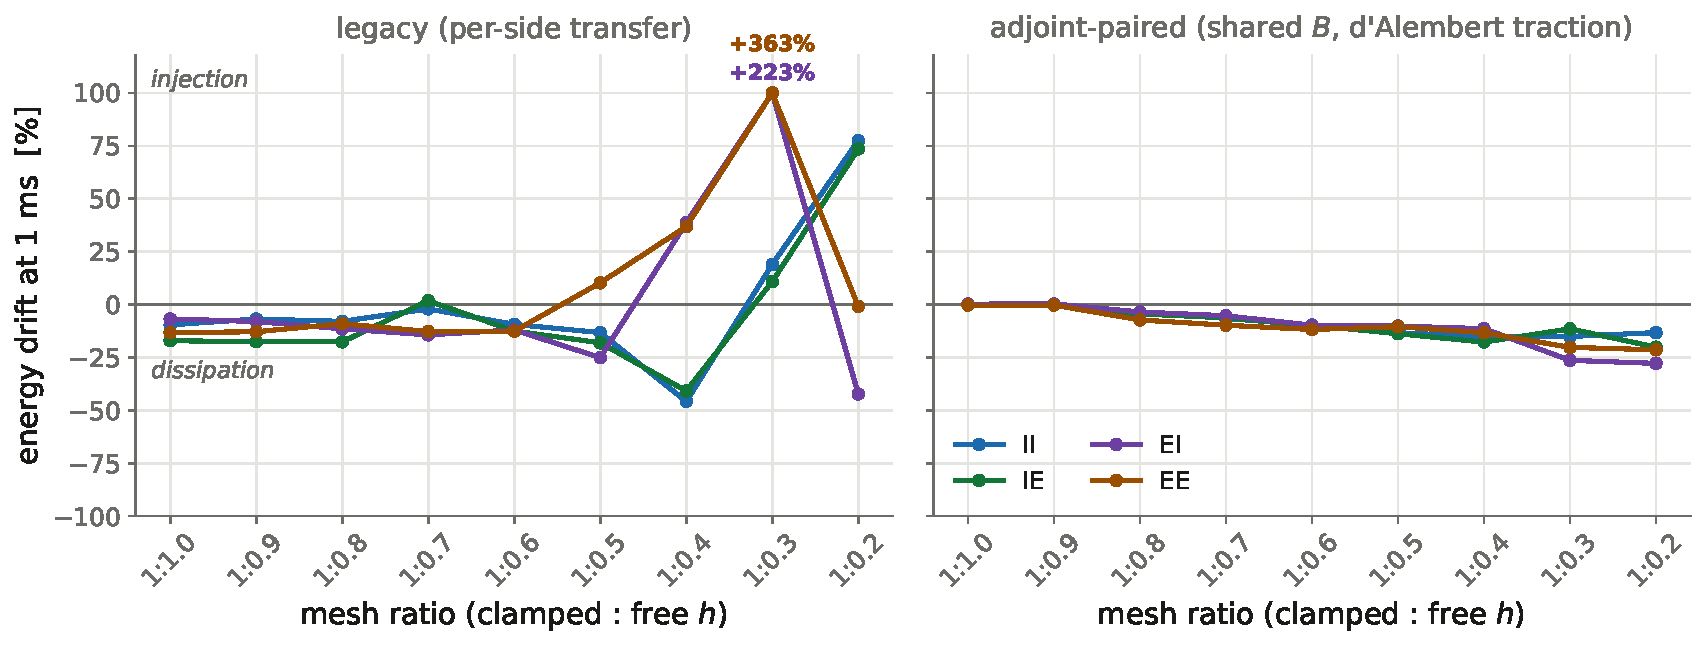
\includegraphics[width=\textwidth]{figs/legacy-vs-paired.pdf}
\caption{Nonoverlap impedance Schwarz, energy drift at 1\,ms across the
mesh-ratio family, all four integrator combinations. Left: legacy per-side
transfer (consistent-mass integer-step metric) --- sign-indefinite, with
injection up to $+363\%$ (EE) and $+223\%$ (EI) at $1{:}0.3$. Right: the
adjoint-paired coupling (staggered lumped-mass metric of
Eq.~\eqref{eq:staggered} for explicit members) --- monotone, sign-definite
trace-jump dissipation at every ratio, and conservation to $\le 0.3\%$ on
conforming and $1{:}0.9$ meshes.}
\label{fig:legacy-paired}
\end{figure}

Table~\ref{tab:legacy-paired} and Fig.~\ref{fig:legacy-paired} compare the
two couplings. Three properties, in order of importance. First, \emph{no
injection at any ratio}: the interface work is sign-definite, as the
telescoping identity \eqref{eq:telescope} guarantees. Second,
near-conservation through mild contrast ($-0.03\%$ at $1{:}0.9$, where
every other variant tested loses or gains several percent). Third, the
residual dissipation at strong contrast is the genuine trace-space jump
being absorbed at rate $Z\!\int_\Gamma \jump{\dot{~u}}^2$: at the exactly
nested ratio $1{:}0.5$ (where the legacy transfer is coincidentally adjoint
and the quadrature is exact) paired and legacy agree to $0.1\%$, so the
remaining loss is not a transfer artifact but the representability price of
Sec.~\ref{sec:ghn} --- now paid in a controlled, monotone, sign-definite
form.

\subsection{Explicit subdomains: IMEX interface treatment}
\label{sec:imex}

With an explicit (central-difference) subdomain on either side, the paired
coupling is strongly unstable ($+10^3$ to $+10^5\,\%$) if the interface
terms are evaluated at lagged time levels: the consistent traction couples
the partner's \emph{acceleration} into the interface force, an algebraic
loop that the implicit pairs resolve within the Schwarz iteration. The cure
is the implicit--explicit (IMEX) structure of Liu et al.: because the
dashpot force is linear in the unknown acceleration, the explicit update is
closed implicitly on the interface rows only,
\begin{equation}
  \bigl(~M + \gamma\,\Delta t\,Z\,W\bigr)\big|_\Gamma\, ~a_{n+1}
  \;=\; ~M\,~a^{\mathrm{expl}}\big|_\Gamma,
  \label{eq:imex}
\end{equation}
a small symmetric-positive-definite solve per interface (reused for the
three components) while the interior stays matrix-free explicit
(\code{imex\_interface\_acceleration!}); the dashpot then acts on the
end-of-step velocity and the Schwarz iteration synchronizes both sides at
$t_{n+1}$ exactly as in the implicit--implicit case.

\begin{table}[htbp]
\centering
\caption{Energy drift at 1\,ms of the adjoint-paired nonoverlap coupling,
all integrator combinations, staggered metric \eqref{eq:staggered} for
explicit members, in percent.}
\label{tab:paired-all}
\begin{tabular}{lrrrr}
\toprule
ratio & II & IE & EI & EE \\
\midrule
1:1.0 & $-0.03$ & $-0.11$ & $+0.20$ & $-0.27$ \\
1:0.9 & $-0.03$ & $-0.10$ & $+0.29$ & $-0.27$ \\
1:0.8 & $-3.6$ & $-4.4$ & $-3.5$ & $-7.3$ \\
1:0.7 & $-6.6$ & $-6.2$ & $-5.3$ & $-9.8$ \\
1:0.6 & $-9.7$ & $-9.8$ & $-9.8$ & $-11.8$ \\
1:0.5 & $-13.3$ & $-13.8$ & $-10.2$ & $-10.5$ \\
1:0.4 & $-15.1$ & $-17.8$ & $-11.4$ & $-13.3$ \\
1:0.3 & $-15.1$ & $-11.5$ & $-26.4$ & $-20.2$ \\
1:0.2 & $-13.3$ & $-20.1$ & $-27.8$ & $-21.4$ \\
\bottomrule
\end{tabular}
\end{table}

On conforming and mildly nonconforming meshes all four integrator
combinations conserve to $\le 0.3\%$ (Table~\ref{tab:paired-all}); the
nonconforming columns carry the same monotone, sign-definite trace-jump
dissipation in every combination. (The small positive EI entries,
$+0.2$--$0.3\%$, are bounded transient storage in the conservative
interface spring, not secular growth.) In the consistent-mass integer-step
metric the explicit columns instead read $-4$ to $-37\%$; the difference is
the metric artifact of Sec.~\ref{sec:benchmark}, not the coupling ---
against the monodomain explicit reference the conforming paired EE
trajectory is exact to $0.35\%$ \emph{pointwise over the whole
millisecond}: the coupled trajectory is the monodomain trajectory, as the
fixed-point argument predicts.

\section{Subcycling: different time steps per subdomain}
\label{sec:subcycle}

Different time steps per subdomain require no new exchange machinery: each
subdomain records its per-substep trajectory (kinematics and internal
force) during every Schwarz iteration, the coupling evaluates the partner's
state in time at each of its own substeps, and the paired d'Alembert
traction follows. (Enabling this exposed a time-step erosion defect in the
subcycler --- the stop-aligned remainder step persisted as the nominal step
and the Schwarz re-integration amplified the floating-point remainder
geometrically --- fixed independently of the pairing.)

\subsection{Genuine interpolation}
\label{sec:gc}

The exchange was intended to interpolate the partner piecewise-linearly in
time --- the interpolated-continuity structure under which
Gravouil--Combescure prove the subcycled interface work dissipative
($E_{\mathrm{int}} \le 0$, $O(\Delta t)$) --- but two infrastructure defects
meant that is not what actually ran. First, the history interpolation
selected the wrong segment (an off-by-one error that returned the
end-of-history value for any query in the last segment and extrapolated
backward elsewhere). Second, the per-stop history was anchored at the first
substep, not the stop start, so a non-subcycling partner's history was a
single end-of-stop entry. Net effect: both directions of the exchange
end-sampled the partner's stop-end state --- constant, not interpolated,
data. With both defects fixed the exchange is genuinely piecewise-linear in
both directions. Table~\ref{tab:subcycled} compares the two at $1$\,ms with
the free side subcycled $4{:}1$ ($\Delta t = 0.25\,\mu$s inside a $1\,\mu$s
stop; consistent-mass integer-step metric for comparability across the
development history).

\begin{table}[htbp]
\centering
\caption{Energy drift at 1\,ms of the subcycled ($4{:}1$) adjoint-paired
coupling with the defective end-sampled exchange vs.\ the corrected
piecewise-linear interpolation, in percent (consistent-mass integer-step
metric).}
\label{tab:subcycled}
\begin{tabular}{lrr}
\toprule
case & end-sampled (defective) & interpolated (fixed) \\
\midrule
conforming II & $-2.8$ & $-3.6$ \\
conforming IE & $-9.6$ & $-10.1$ \\
conforming EE & $-10.6$ & $-9.6$ \\
1:0.5 II & $-20.6$ & $\mathbf{-14.1}$ \\
1:0.5 IE & $-24.4$ & $\mathbf{-21.3}$ \\
\bottomrule
\end{tabular}
\end{table}

(In the staggered metric the interpolated exchange reads conforming II
$-3.6$, IE $-1.4$, EE $-1.2\%$: the explicit subcycled overhead is about
one percent on conforming meshes.) Genuine interpolation is clearly better
at mesh contrast, where end-sampling aliases the fine side's intra-window
motion into the exchanged traction. It loses slightly on the conforming
implicit cases because the end-sampled datum, being the stop-end value
applied throughout the window, \emph{leads} the true trajectory, and that
anticipatory bias is a mild energy-injection channel that happened to
offset part of the interpolation dissipation. A cancellation between two
discretization errors is not a conservation property, and this one fails
precisely at strong mesh contrast; the interpolated exchange is the
behavior of the paired coupling.

\subsection{Exact telescoping is incompatible with a partitioned exchange}
\label{sec:ph}

Prakash--Hjelmstad telescope the subcycled interface work to exactly zero
by giving the interface traction a linear-in-time representation whose step
values satisfy
$\tfrac12(\hat\lambda_n + \hat\lambda_{n+1})
 = \overline{\lambda}_{n \to n+1}$
(the partner's window average), so the trapezoidal work sums of the two
sides cancel window by window. Three Schwarz-compatible constructions of
this datum were implemented and measured:

\begin{description}
  \item[Window average.] Handing the coarse side the partner's trapezoidal
  window average is work-conjugate to the fine side's interpolation --- but
  an average estimates the window midpoint, and the half-window lag of the
  interface force behind the interface motion is artificial damping:
  uniformly worse than plain interpolation ($-3.6 \to -4.2$,
  $-10.1 \to -11.1$, $-9.6 \to -12.3$, $-14.1 \to -15.5$,
  $-21.3 \to -23.0$).
  \item[Exact telescoping recursion.] The lag-free datum
  $\hat\lambda_{n+1} = 2\overline{\lambda} - \hat\lambda_n$ satisfies the
  telescoping identity exactly --- and diverges: the factor of two on the
  partner-state channel doubles the Schwarz iteration's contraction factor,
  and the coupled iteration diverges within tens of stops.
  \item[Least-squares endpoint fit.] The endpoint value of the
  least-squares linear fit of the partner trajectory over the window is
  lag-free, filters intra-window content instead of aliasing it, and
  telescopes for window-linear tractions. It is stable over tens of stops
  and passes the short regression test --- and over hundreds of stops it
  injects energy catastrophically ($+10^3$--$10^5\%$ before aborting): a
  zero-lag filtered estimate is an extrapolation, and its frequency
  response exceeds unity outside the linear band.
\end{description}

The pattern is the classical stability principle of partitioned coupling:
only \emph{causal} transfer operators (lag $\ge 0$) are robust in a
fixed-point exchange, and every zero-lag work-conjugate datum is
anticipatory. Prakash--Hjelmstad's telescoping is consistent with this ---
their method solves the coupled interface problem \emph{directly} (a
FETI-style interface system per large step), which is precisely what a
partitioned Schwarz sweep does not do. Exact subcycled interface-work
telescoping therefore requires a direct interface solve, not a modified
partitioned exchange; within the Schwarz family, genuinely interpolated
Gravouil--Combescure transfer is the measured stable optimum, and its
$O(\Delta t)$ dissipation ($-3.6\%$ at conforming II vs.\ $-0.03\%$
same-step) is the price of subcycling. (The window-average and
endpoint-fit utilities remain in \code{interpolation.jl} as tested
building blocks.)

\section{Long-horizon behavior}
\label{sec:tenms}

Every conclusion above rests on $1$\,ms runs --- about two transits of the
release front. To test which behaviors are steady and which are transients,
all $151$ study configurations were rerun to $10$\,ms ($10^4$ stops): the
full overlap sweep, the nonoverlap paired sweep and its subcycled set, and
fresh monodomain references. Both monodomain references conserve the
staggered energy \eqref{eq:staggered} to $\pm 0.000\%$ over the full
$10$\,ms, and every surviving run reproduces its recorded $1$\,ms drift at
its $t = 1$\,ms row.

\subsection{Overlap: the 1\,ms drifts were transients of instabilities}

The overlap family is long-horizon unstable almost everywhere. Of the $108$
overlap runs, $74$ were terminated by element inversion after exponential
energy growth (typically $+3{,}000$ to $+10{,}000\%$ of $E_0$ at failure,
between $2$ and $9$\,ms), and most of the remainder collapsed toward zero
energy. The sign-indefinite drifts of the $1$\,ms sweep were early sections
of these trajectories: configurations that appeared dissipative at $1$\,ms
(e.g.\ maximum overlap $1{:}0.6$ II, $-61\%$) reversed and grew to
$+5{,}432\%$ at failure. Mesh conformity does not save the mixed-integrator
combinations: the conforming half-overlap IE run read $+13\%$ at $1$\,ms,
grew exponentially, and failed at $6.25$\,ms; conforming EI behaves alike
at all three widths. The only overlap configurations that remain stable and
accurate at $10$\,ms are the conforming II runs: $+0.64$, $+0.61$,
$+0.16\%$ at the three overlap widths (Fig.~\ref{fig:overlap-10ms}). The
overlap coupling is therefore a short-horizon method on nonconforming
meshes, and for non-II combinations even on conforming ones.

\begin{figure}[htbp]
\centering
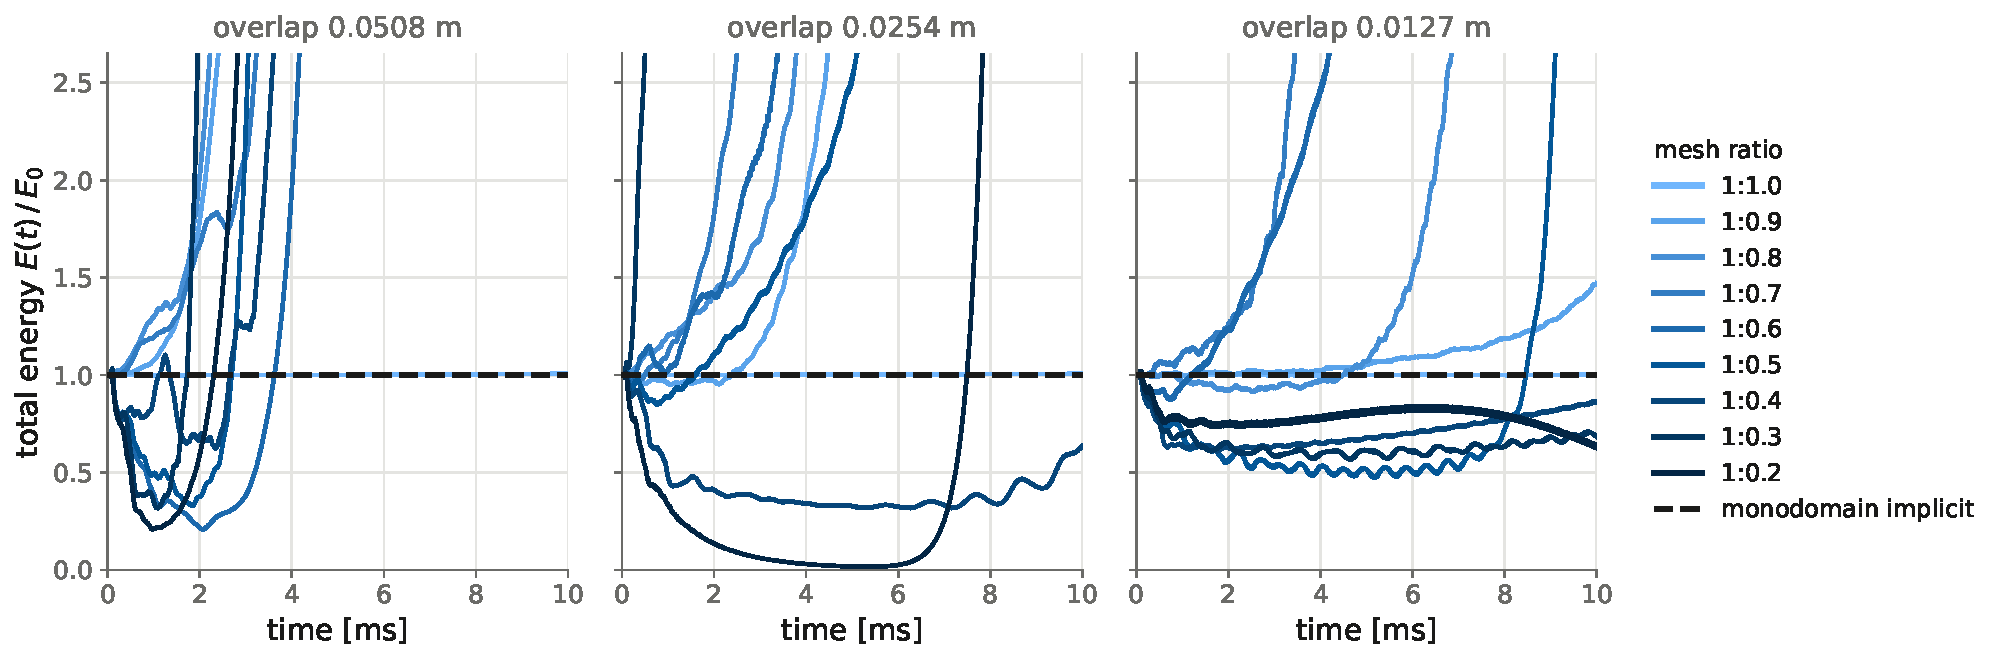
\includegraphics[width=\textwidth]{figs/overlap-II-10ms.pdf}
\caption{Overlap impedance Schwarz (variational transfer),
implicit--implicit, $10$\,ms horizon. Nearly every nonconforming
configuration either grows exponentially until element inversion ends the
run (curves leaving the top of the axes) or collapses toward zero energy;
only the conforming ($1{:}1.0$) runs track the monodomain reference. The
mixed and all-explicit combinations (not shown) are worse: they lose even
the conforming cases.}
\label{fig:overlap-10ms}
\end{figure}

\subsection{Nonoverlap pairing: no injection, but compounding dissipation
and two new failure modes}

The paired nonoverlap coupling never injects at any ratio in any
combination, at $10$\,ms as at $1$\,ms. Its monotone trace-jump
dissipation, however, compounds (Table~\ref{tab:nonoverlap-10ms}).

\begin{table}[htbp]
\centering
\caption{Energy drift at 10\,ms of the adjoint-paired nonoverlap coupling,
staggered metric, in percent. $\dagger\,t$: run terminated by element
inversion at $t$\,ms. $\ast$: run ended in the noise-saturated
explicit--explicit state discussed in the text.}
\label{tab:nonoverlap-10ms}
\begin{tabular}{lrrrr}
\toprule
ratio & II & IE & EI & EE \\
\midrule
1:1.0 & $+0.00$ & $-0.9$ & $-0.2$ & $\ast$ \\
1:0.9 & $+0.00$ & $-0.5$ & $+0.1$ & $\ast$ \\
1:0.8 & $\dagger\,5.2$ & $\dagger\,3.9$ & $\dagger\,4.0$ & $\dagger\,2.6$ \\
1:0.7 & $\dagger\,4.9$ & $\dagger\,3.7$ & $\dagger\,3.9$ & $\dagger\,2.8$ \\
1:0.6 & $-47.3$ & $-56.4$ & $-42.9$ & $\ast$ \\
1:0.5 & $-56.8$ & $-72.0$ & $-40.8$ & $\ast$ \\
1:0.4 & $-54.9$ & $-73.9$ & $-40.4$ & $\ast$ \\
1:0.3 & $-65.1$ & $-66.0$ & $-81.1$ & $\ast$ \\
1:0.2 & $-53.3$ & $-73.1$ & $-84.1$ & $\ast$ \\
\bottomrule
\end{tabular}
\end{table}

\begin{figure}[htbp]
\centering
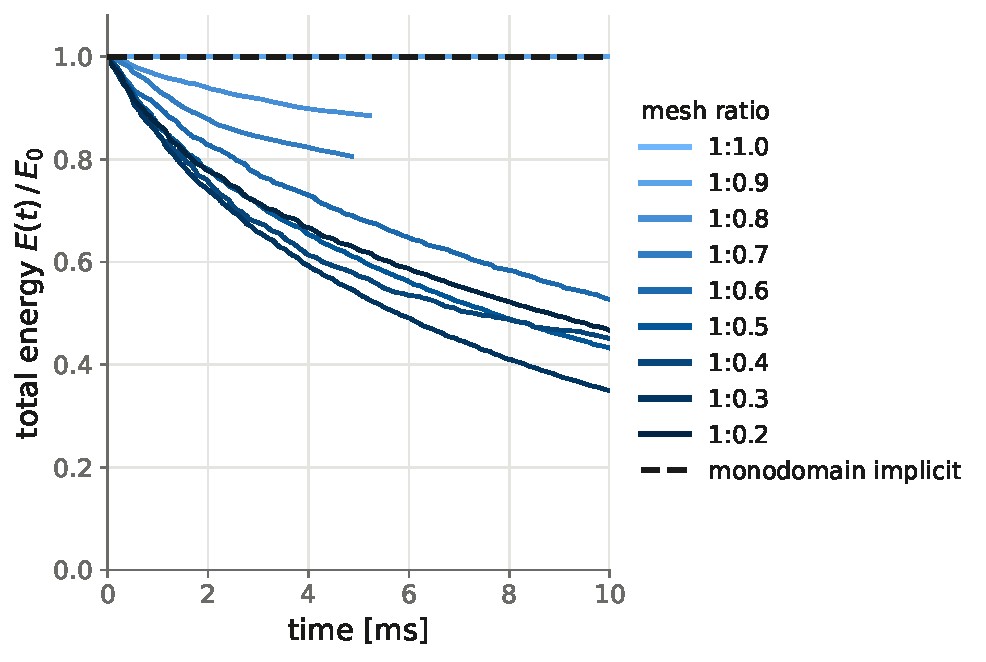
\includegraphics[width=0.495\textwidth]{figs/nonoverlap-II-10ms.pdf}\hfill
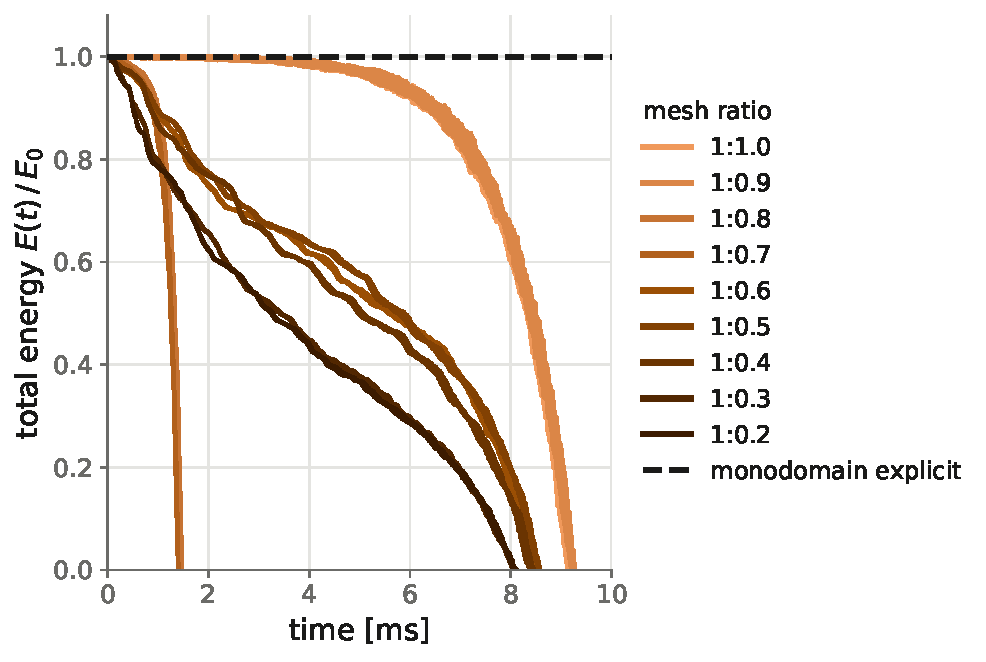
\includegraphics[width=0.495\textwidth]{figs/nonoverlap-EE-10ms.pdf}
\caption{Adjoint-paired nonoverlap impedance Schwarz, $10$\,ms horizon,
staggered energy metric. Left: implicit--implicit --- no injection
anywhere; conforming and $1{:}0.9$ hold the monodomain reference, strong
contrast dissipates monotonically, and the non-nested ratios
$1{:}0.7$--$1{:}0.8$ end early at $\approx 5$\,ms (interface element
inversion). Right: explicit--explicit --- the staggered kinetic term goes
secularly negative at every ratio as undamped grid-frequency content
accumulates at $\mathrm{CFL}=1$; the $1{:}0.7$--$1{:}0.8$ runs fail by
central-difference instability at $2.6$--$2.8$\,ms.}
\label{fig:nonoverlap-10ms}
\end{figure}

Three observations (Fig.~\ref{fig:nonoverlap-10ms}). First, with an
implicit member the conforming and $1{:}0.9$ columns hold $0.00$ to
$-0.9\%$ over ten thousand stops. Second, at strong contrast
($\le 1{:}0.6$) the sign-definite dissipation that read as $10$--$28\%$ at
$1$\,ms reaches $40$--$85\%$ by $10$\,ms: bounded and ordered, but far too
large for wave-transit accuracy. Absorption of unrepresentable content is a
rate, not a one-time toll. Third, the mildly nonconforming, \emph{non-nested}
ratios $1{:}0.7$ and $1{:}0.8$ form a failure window invisible at $1$\,ms:
the paired transfer accumulates interface-local high-frequency displacement
content, and every integrator combination eventually fails there ---
explicit members at $2.6$--$4$\,ms by central-difference instability,
implicit pairs at $\approx 5$\,ms when the first interface element inverts
while the global energy is still smooth ($-19\%$ at failure). This is not a
relaxation artifact: reruns with fixed $\theta = 0.5$ fail identically
(trajectories matching to three digits), so the noise accumulation belongs
to the transfer operators themselves. The nested ratios ($1{:}0.5$ exactly,
and the strong ratios whose transfer filters aggressively) do not exhibit
it.

\subsection{Explicit--explicit saturation, and subcycling as a remedy}

The EE column degrades at every ratio by $10$\,ms, conforming included,
ending with the staggered metric near $-2\,E_0$. The end state is not a
divergence: the stored energy stays bounded and physical throughout (the
conforming run holds $E/E_0 \ge 0.97$ to $5$\,ms, then declines), but the
staggered kinetic term goes steadily negative --- the signature of sawtooth
content at $\omega\Delta t \approx 2$ accumulating in velocity and
acceleration. Central difference at $\mathrm{CFL} = 1$ has zero numerical
dissipation at the stability limit, so whatever grid-frequency content the
interface exchange seeds is never removed; with no implicit member in the
pair, it accumulates without bound in amplitude-neutral modes. The measured
remedy is time-step margin: the subcycled conforming EE run (free side at
$\Delta t/4$, $\mathrm{CFL} = 0.25$) ends at $-10.8\%$ with no saturation.
Subcycling has the opposite effect on the implicit--implicit pair: the
same-step conforming II run conserves to $+0.00\%$ while the subcycled one
loses $-20.2\%$ (at $1{:}0.5$, $-61.6\%$) --- the Gravouil--Combescure
interpolation dissipation of Sec.~\ref{sec:gc}, harmless per stop,
compounds over $10^4$ stops. At long horizons the multi-time-step exchange
is thus a trade: it stabilizes explicit members (CFL margin) and taxes
implicit ones (interpolation dissipation). Figure~\ref{fig:subcycled-10ms}
shows both sides of the trade.

\begin{figure}[htbp]
\centering
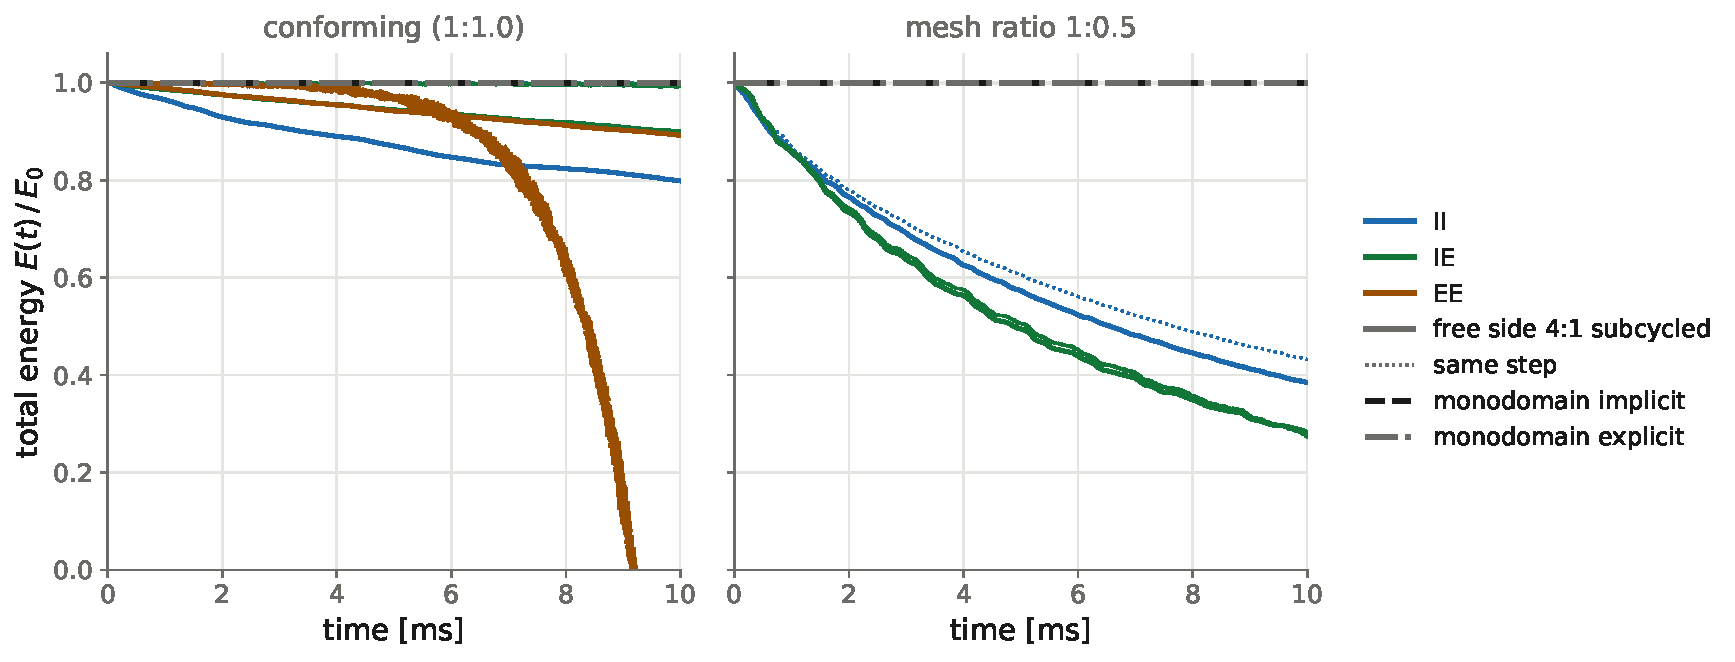
\includegraphics[width=\textwidth]{figs/nonoverlap-subcycled-10ms.pdf}
\caption{Subcycled (free side $4{:}1$, solid) vs.\ same-step (dotted)
adjoint-paired nonoverlap coupling over $10$\,ms. Left, conforming: the
subcycled EE run (orange solid, $\mathrm{CFL}=0.25$) avoids the saturation
that destroys same-step EE (orange dotted), while subcycled II (blue solid)
pays the compounding interpolation dissipation that same-step II (on the
reference line) does not. Right, mesh ratio $1{:}0.5$: at strong contrast
the trace-jump dissipation dominates and the subcycling overhead is
comparatively small (II subcycled $-61.6\%$ vs.\ same-step $-56.8\%$).}
\label{fig:subcycled-10ms}
\end{figure}

The long-horizon ranking is unambiguous: adjoint-paired nonoverlap coupling
with at least one implicit interface member, on conforming or nested mesh
ratios, is the only tested configuration that is sound at $10$\,ms; the
overlap family is short-horizon only.

\section{Windowed controller stops and the relaxation state}
\label{sec:windowed}

The multi-domain controller advances in \emph{stops}; within a stop each
subdomain subcycles to the stop end with its own time step, and partner
data are exchanged as per-substep trajectories with piecewise-linear time
interpolation (Sec.~\ref{sec:subcycle}). With the subdomain steps held
fixed ($1\,\mu$s), does the controller stop size --- the window over which
the Schwarz iteration converges before committing --- affect the converged
physics? A sweep over windows of $1$ (baseline), $2$, $5$, and $10\,\mu$s
on representative overlap and nonoverlap cases, run to $10$\,ms, gave a
split answer.

\paragraph{Overlap: a pure cost parameter.} Every overlap trajectory is
identical across all four windows to all printed digits --- the conforming
II run ends at $+0.61\%$ in all four, and the $1{:}0.5$ instability even
fails at the same instant. The overlap exchange interpolates partner
kinematics from history with no per-pair relaxation state, so the windowed
waveform iteration converges to the same-step fixed point.

\paragraph{Nonoverlap: the window shifted the fixed point.} Drift for the
conforming paired II case at $10$\,ms: $+0.00\%$ same-step, $+11.3\%$ at
the $2\,\mu$s window, $-81.9\%$ at $5\,\mu$s, $-83.7\%$ at $10\,\mu$s
(Aitken relaxation; with fixed $\theta = 0.5$ the sequence is a monotone
drain instead, $-7.1\%$ at $2\,\mu$s to $-87.9\%$ at $10\,\mu$s). This was
not a convergence failure --- the sweeps converged normally --- but a
defect of the relaxation machinery: the relaxation state ($\lambda$ vectors
and Aitken residual buffers) was stored as one vector per interface pair,
updated on every boundary-condition application. In a windowed stop the
relaxed side of a pair (the later-listed member) applies its coupling
condition once per \emph{substep}, so the blend
$(1-\theta)\,g + \theta\,\mathrm{rhs}$ mixed iterates across \emph{time}
rather than across Schwarz sweeps: a causal exponential low-pass filter
(lag $\sim \Delta t_{\mathrm{sub}}/\theta$) on the exchanged traction,
whose lag dissipation grows with the window. Under Aitken the defect
changes sign: the $\theta$ estimate compares residuals belonging to
different times, overshoots past $1$, and the resulting phase lead injects
energy --- the $+11.3\%$ entry. (The subcycled study of
Sec.~\ref{sec:subcycle} was unaffected because its subcycling free side is
listed first and therefore unrelaxed.)

Two experiments isolate and confirm the mechanism. First, $\theta = 1$ ---
which uses no relaxation state at all --- reproduces the same-step physics
on the unmodified code at every window ($+0.00\%$ over the full $10$\,ms at
the $10\,\mu$s window). Second, with the fix below in place, all windowed
policies land on the same-step trajectory. The fix keys the relaxation
state by pair \emph{and} by substep time slot within the current stop,
clearing it at every stop (\code{relaxation\_slot!} in \code{schwarz.jl});
with one substep per stop it reduces exactly to the classical per-pair
iteration, and the same-step code path is bit-identical to the pre-fix
baselines. Windowed runs then match same-step to Schwarz truncation (the
residual $3.9\times 10^{-6}$ displacement mismatch at working tolerances
collapses to $3.7\times 10^{-8}$ as the stopping tolerances tighten), and a
windowed-equivalence regression guards this in the adjoint-pairing test
(test 109).

\begin{figure}[htbp]
\centering
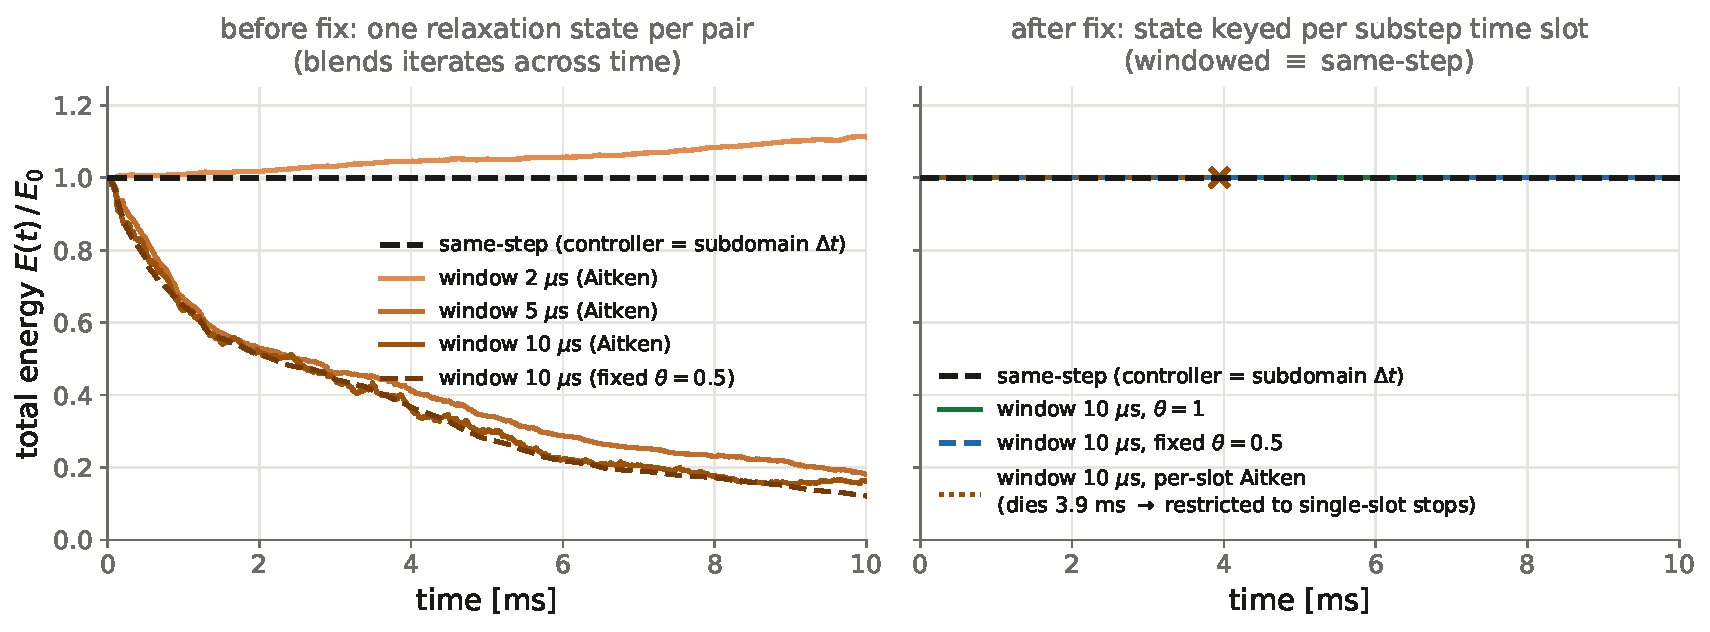
\includegraphics[width=\textwidth]{figs/windowed-stops.pdf}
\caption{Windowed controller stops on the conforming paired II case,
$10$\,ms. Left, pre-fix: the per-pair relaxation state blends iterates
across time --- Aitken injects at the $2\,\mu$s window and drains at
$5$--$10\,\mu$s; fixed $\theta = 0.5$ drains monotonically. Right, post-fix
(slot-keyed state): every windowed policy lands on the same-step
trajectory; the per-slot Aitken run is physically correct until its
unclamped $\theta$ excursions cause a Newton failure at $3.9$\,ms
($\times$), which motivated restricting Aitken to single-slot stops.}
\label{fig:windowed}
\end{figure}

\paragraph{Relaxation policy inside windows.} With the state fixed, the
remaining question is which relaxation policy a windowed stop should use.
Measured on the conforming II case at the $10\,\mu$s window (mean Schwarz
sweeps per stop): $\theta = 1$ converges in $19.1$ and runs the full
$10$\,ms without incident; per-slot Aitken takes ${\sim}25$ and fails at
$3.9$\,ms when an unclamped $\theta$ excursion causes the Newton iteration
to diverge; fixed $\theta = 0.5$ takes $47.5$ (no failures); and a
waveform-pooled Aitken (one $\theta$ from residuals pooled across the
window's slots) takes $55.1$ --- no failures on II but it fails on EE,
where it locks $\theta$ persistently negative. Aitken acceleration
therefore offers no benefit inside windows and can cause failure, and Norma
applies it only to single-slot stops, where its ${\approx}3\times$ sweep
reduction is established (\code{aitken\_applies}); windowed stops use the
configured \code{relaxation parameter}, with $\theta = 1$ recommended ---
the impedance dashpot supplies the contraction, so no under-relaxation is
needed.

Two limitations complete the picture. The all-explicit pair at large
windows is impractical under any policy: the windowed explicit sweep map is
nearly non-contractive (fixed $\theta = 0.5$ reaches the $128$-sweep limit
and still fails at $9.8$\,ms). And windows are never a cost optimization
for the nonoverlap exchange: the number of substep solves per unit time is
(sweeps per stop)$/\Delta t_{\mathrm{sub}}$ regardless of the window, and
the windowed sweep counts above all exceed the same-step Aitken count, so
the controller step is purely a convenience parameter (e.g.\ for aligning
output stops), cost-neutral at best. For the overlap family, by contrast,
larger stops are a mild speedup (fewer, marginally more iterated stops).
One earlier observation is withdrawn as an artifact: the pre-fix ``EE at
the $2\,\mu$s window with fixed $\theta$ ends at $-0.25\%$'' entry was the
defect's low-pass filter accidentally damping the grid-frequency
saturation; post-fix, windowed EE saturates exactly like same-step EE, and
the effective remedy remains CFL margin via subcycling
(Sec.~\ref{sec:tenms}).

\paragraph{Open issue: a $\theta$-sensitive fixed point.} The
windowed-equivalence test exposed a pre-existing defect, orthogonal to the
fix: the \emph{converged} paired-impedance solution depends weakly on the
relaxation parameter --- $\theta = 0.5$ and $\theta = 1.0$ differ by
${\sim}4\times 10^{-5}$ relative displacement on the $2{:}1$ nonconforming
cantilever at a $10^{-13}$ stopping tolerance, same-step and windowed
alike, and an Aitken run lands on the $\theta = 1$ answer to $10^{-12}$.
Instrumentation rules out the blend algebra (the blended base is
identically zero at interface degrees of freedom, because \code{apply\_bcs}
zeroes the boundary force before each pass); the evidence points to a
neutral --- non-contracting --- mode of the paired exchange that retains
its $\theta$-dependent initialization and is invisible to the
displacement-based stopping criterion. The magnitude is far below every
signal in this study ($\ge 10^{-4}$), but it is a genuine correctness
question and needs its own investigation.

\section{Conclusions and recommendations}
\label{sec:conclusion}

\subsection{Summary of findings}

\begin{enumerate}[itemsep=2pt]
\item On a shared interface, Robin coupling is fully reflecting
  ($\lvert R \rvert \equiv 1$) and the impedance condition is absorbing
  ($\lvert R \rvert < 1$, zero at $\alpha = 0$) with the impedance fixed by
  material data; in the quasi-static limit the impedance condition
  collapses onto Robin (Sec.~\ref{sec:nonoverlap-tc}).
\item On an overlap boundary, the impedance condition is consistent with
  the monodomain solution only with the partner-traction term, and the
  quality of that traction sets the conforming energy error:
  $59\% \to 14\% \to 1.5\% \to 0.08\%$ over $1$\,ms as the traction
  evaluation improves to the consistent nodal reaction, with no adjustable
  parameters (Sec.~\ref{sec:ladder}).
\item On nonconforming overlap decompositions the coupling family is
  absorbing-or-unstable: Dirichlet matching (pointwise or weak) is severely
  unstable, and the impedance condition is stable precisely because its
  dashpot continually absorbs the inter-grid disagreement, whose dominant
  component is coarse-grid dispersion --- a smooth, in-band solution defect
  that neither spatial filtering nor any measured increase in transfer
  fidelity can close at fixed $h$ (Secs.~\ref{sec:fidelity},
  \ref{sec:study}).
\item The interface work of the overlap coupling is sign-indefinite in
  principle (two independent, non-adjoint transfers) and in practice
  (injection up to $+275\%$; sign flips between adjacent mesh ratios), and
  at a $10$\,ms horizon $74$ of $108$ nonconforming overlap runs fail. The
  nonconforming overlap coupling cannot be assigned a reliable energy
  budget (Secs.~\ref{sec:ratiosweep}, \ref{sec:tenms}).
\item Energy consistency requires a single-valued interface traction acting
  through $L^2$-adjoint transfer operators built from one cross-mass matrix
  --- then the interface power telescopes to a sign-definite dissipation on
  the interface jump \eqref{eq:telescope}. This is implementable only on
  the nonoverlap variant, which has a shared interface
  (Sec.~\ref{sec:theory}).
\item The adjoint-paired nonoverlap coupling --- d'Alembert interface
  reaction, shared cross-mass matrix, harmonic-mean pair impedance, IMEX
  interface rows for explicit subdomains --- never injects at any mesh
  ratio in any integrator combination, conserves to $\le 0.3\%$ at $1$\,ms
  on conforming and mildly nonconforming meshes in all four combinations,
  and reproduces the monodomain trajectory pointwise
  (Sec.~\ref{sec:paired}).
\item At long horizons the paired coupling's sign-definite dissipation at
  strong mesh contrast compounds ($40$--$85\%$ at $10$\,ms); the non-nested
  ratios $1{:}0.7$--$1{:}0.8$ accumulate interface-local high-frequency
  content until an interface element inverts; and the all-explicit pair at
  $\mathrm{CFL} = 1$ saturates with undamped grid-frequency content, for
  which subcycling (CFL margin) is an effective remedy
  (Sec.~\ref{sec:tenms}).
\item Subcycling uses genuine piecewise-linear interpolation of partner
  trajectories (two silent defects that reduced it to end-sampling are
  fixed); its $O(\Delta t)$ dissipation is the price of subcycling, and
  exact interface-work telescoping is structurally incompatible with a
  partitioned exchange --- it requires a direct interface solve
  (Sec.~\ref{sec:subcycle}).
\item The Schwarz relaxation state must be keyed per pair and per substep
  time slot; otherwise controller stops larger than a subdomain step blend
  iterates across time and shift the converged fixed point. With the
  slot-keyed state, windowed stops are equivalent to same-step to Schwarz
  truncation, and the controller step is a pure convenience parameter.
  Aitken acceleration applies only to single-slot stops; windowed stops
  should use $\theta = 1$ (Sec.~\ref{sec:windowed}).
\end{enumerate}

\subsection{Practical recommendations}

\begin{itemize}[itemsep=2pt]
\item \textbf{Energy-critical dynamic coupling}: use the adjoint-paired
  nonoverlap impedance variant (the default for \code{Schwarz impedance
  nonoverlap}) with at least one implicit interface member and a conforming
  or nested mesh ratio. Avoid the non-nested mild ratios
  ($1{:}0.7$--$1{:}0.8$ class) for long runs.
\item \textbf{Overlap decompositions}: conforming meshes with
  implicit--implicit integration conserve energy at any horizon; every
  other overlap configuration is suitable for short transients only. On
  conforming node-aligned interfaces the consistent traction makes the
  impedance overlap condition exact to the Dirichlet-coupling reference.
\item \textbf{All-explicit interfaces}: provide CFL margin (e.g.\ subcycle
  the finer side); central difference at $\mathrm{CFL} = 1$ cannot remove
  the grid-frequency content the exchange seeds.
\item \textbf{Parameters}: no impedance tuning anywhere --- the impedance
  is material data (harmonic mean per pair for nonoverlap; partner material
  with P/S split for overlap). The Robin parameter affects only the
  iteration, not the converged solution, and must be a single value per
  interface under pairing. Historical per-problem tuning of impedance
  scales and large Robin values is obsolete.
\item \textbf{Diagnostics}: use the blended (partition-of-unity) energy
  output and the staggered metric \eqref{eq:staggered} for explicit
  members; use the channel-resolved interface-work instrumentation as the
  acceptance metric for any change to the transmission machinery --- a
  small net drift can be a cancellation of large opposing channels.
\item \textbf{Robustness at fixed cost} on nonconforming overlap runs that
  cannot be avoided: mild HHT-$\alpha$ damping
  ($\bar\alpha \approx 0.02$--$0.05$) converts sign-indefinite drift into
  monotone decay, at a cost proportional to the energy in the reverberating
  band.
\end{itemize}

\subsection{Open questions}

(i) The weakly $\theta$-sensitive fixed point of the paired exchange
(${\sim}4\times 10^{-5}$ relative displacement), evidence of a neutral mode
invisible to the displacement-based stopping criterion
(Sec.~\ref{sec:windowed}). (ii) The non-nested mesh-ratio failure window of
the paired transfer at long horizons (Sec.~\ref{sec:tenms}). (iii) Exact
subcycled telescoping via a direct FETI-style interface solve, together
with the localized-Lagrange-multiplier frame construction (Park--Felippa;
Dvorak et al.\ 2023) (Sec.~\ref{sec:ph}). (iv) A bimaterial benchmark to
exercise the tensor impedance and the harmonic-mean pair impedance where
they should be most beneficial. (v) A smooth-content benchmark to quantify
the HHT-$\alpha$ robustness/cost trade on problems with scale separation
(Sec.~\ref{sec:hht}).

\subsection*{Data provenance}

Cantilever ladder study and instrumentation:
\code{rigel:\char`~/test/Norma/cantilever-energy}. Parametric study, ratio
sweep, $10$\,ms horizon, controller-step sweep, figures, and run harness:
\code{\char`~/cantilever-energy-study/} (\code{ratio-sweep/},
\code{*-10ms}, \code{controller-step-sweep/}, \code{wccm-plots/},
\code{drift-table-10ms.txt}). Regression tests: 103/104 (overlap
projectors and consistent traction), 105 (content-absorption
dissipativity), 109 (adjoint pairing and windowed equivalence,
\code{test/schwarz-nonoverlap-impedance-adjoint-pairing.jl}).

\end{document}
